% memoire.tex — Document principal du mémoire (≈ 75 pages hors annexes) :
% pages liminaires, introduction, trois parties de taille égale (état de l'art,
% réalisation, résultats), conclusion, bibliographie, annexes.
% Les encadrés jaunes « À rédiger » donnent pour chaque section le contenu
% attendu et le nombre de pages visé ; le chapitre sur le jeu du seau d'eau et
% la méthodologie sont rédigés. Compilation : voir README.md.

\documentclass[11pt, a4paper, openany]{report}
% preambule.tex — Paquets, mise en page, couleurs et commandes du mémoire.
% Compilation : pdflatex + biber (Overleaf : compilateur pdfLaTeX, biber détecté
% automatiquement ; en local : latexmk -pdf memoire.tex).

\usepackage[T1]{fontenc}
\usepackage[utf8]{inputenc}
\usepackage{lmodern}
\usepackage[french]{babel}
\usepackage{microtype}
\usepackage[a4paper, margin=2.5cm, headheight=14pt]{geometry}
\usepackage{setspace}
\setstretch{1.12}

\usepackage{amsmath, amssymb}
\usepackage[locale=FR]{siunitx}
\usepackage{graphicx}
\usepackage{xcolor}
\usepackage{booktabs, tabularx, array}
\usepackage{enumitem}
\usepackage{csquotes}
\usepackage[font=small, labelfont=bf]{caption}
\usepackage{subcaption}
\usepackage{float}
\usepackage{tikz}
\usetikzlibrary{babel, arrows.meta, positioning, calc, decorations.pathmorphing, shapes.geometric}
\usepackage{pgfplots}
\pgfplotsset{compat=1.18}
\usepackage{algorithm}
\usepackage{algpseudocode}
\usepackage[most]{tcolorbox}
\usepackage{titlesec}
\usepackage{fancyhdr}
\usepackage[backend=biber, style=authoryear-comp, maxcitenames=2, uniquelist=false]{biblatex}
\addbibresource{bibliographie.bib}
\usepackage[hidelinks]{hyperref}
\usepackage[nameinlink, noabbrev, french]{cleveref}

% Couleurs : reprises de l'application (accent bleu, convention des vecteurs)
\definecolor{accent}{HTML}{1976D2}
\definecolor{soft}{HTML}{E3F2FD}
\definecolor{poids}{HTML}{D32F2F}
\definecolor{normale}{HTML}{2E7D32}
\definecolor{tension}{HTML}{8E24AA}
\definecolor{corde}{HTML}{8D6E63}
\definecolor{eau}{HTML}{1E88E5}
\definecolor{metal}{HTML}{546E7A}
\definecolor{brouillon}{HTML}{FFF8E1}
\definecolor{brouillonbord}{HTML}{F9A825}

% Titres de chapitres sobres, numéro en couleur d'accent
\titleformat{\chapter}[display]
  {\normalfont\bfseries\color{accent}}
  {\large\MakeUppercase{\chaptertitlename}\ \thechapter}
  {6pt}
  {\Huge\color{black}}
  [\vspace{2pt}{\color{accent}\titlerule[1.2pt]}]
\titlespacing*{\chapter}{0pt}{-10pt}{24pt}
\titleformat{\section}{\normalfont\Large\bfseries}{\color{accent}\thesection}{0.8em}{}
\titleformat{\subsection}{\normalfont\large\bfseries}{\color{accent}\thesubsection}{0.8em}{}

\pagestyle{fancy}
\fancyhf{}
\fancyhead[L]{\small\nouppercase{\leftmark}}
\fancyhead[R]{\small\thepage}
\renewcommand{\headrulewidth}{0.4pt}
\fancypagestyle{plain}{\fancyhf{}\fancyfoot[C]{\small\thepage}\renewcommand{\headrulewidth}{0pt}}

\setlist{itemsep=0.25em, topsep=0.4em}

% Commandes
\newcommand{\fichier}[1]{\texttt{#1}}
\newcommand{\vect}[1]{\vec{#1}}

% Encadré « à rédiger » du squelette : objectif de la section, contenu attendu,
% nombre de pages visé. Supprimer l'encadré une fois la section rédigée.
\newtcolorbox{arediger}[1]{enhanced, breakable, colback=brouillon, colframe=brouillonbord,
  boxrule=0.6pt, arc=2pt, left=6pt, right=6pt, top=4pt, bottom=4pt,
  fonttitle=\small\bfseries, coltitle=black, title={À rédiger \hfill \(\approx\) #1}}

% Encadré de point clé dans le texte rédigé
\newtcolorbox{pointcle}{enhanced, colback=soft, colframe=accent, boxrule=0.6pt, arc=2pt,
  left=6pt, right=6pt, top=4pt, bottom=4pt}

% Algorithmes en français
\floatname{algorithm}{Algorithme}
\renewcommand{\listalgorithmname}{Liste des algorithmes}
\algrenewcommand\algorithmicrequire{\textbf{Entrée :}}
\algrenewcommand\algorithmicensure{\textbf{Sortie :}}
\algrenewcommand\algorithmicfor{\textbf{pour}}
\algrenewcommand\algorithmicdo{\textbf{faire}}
\algrenewcommand\algorithmicend{\textbf{fin}}
\algrenewcommand\algorithmicif{\textbf{si}}
\algrenewcommand\algorithmicthen{\textbf{alors}}
\algrenewcommand\algorithmicwhile{\textbf{tant que}}


\begin{document}

\pagenumbering{roman}
% 00-page-de-titre.tex — Page de titre (compléter les champs entre crochets).

\begin{titlepage}
  \centering
  \vspace*{1cm}
  {\large\textsc{[Université]} \par}
  \vspace{0.2cm}
  {\large [Faculté — programme de master] \par}
  \vspace{2.5cm}
  {\color{accent}\rule{\linewidth}{1.2pt}\par}
  \vspace{0.6cm}
  {\Huge\bfseries Des simulations interactives pour enseigner la mécanique en première année d'ingénieur civil \par}
  \vspace{0.4cm}
  {\Large Conception assistée par IA, ludification et évaluation \par}
  \vspace{0.6cm}
  {\color{accent}\rule{\linewidth}{1.2pt}\par}
  \vspace{1.5cm}
  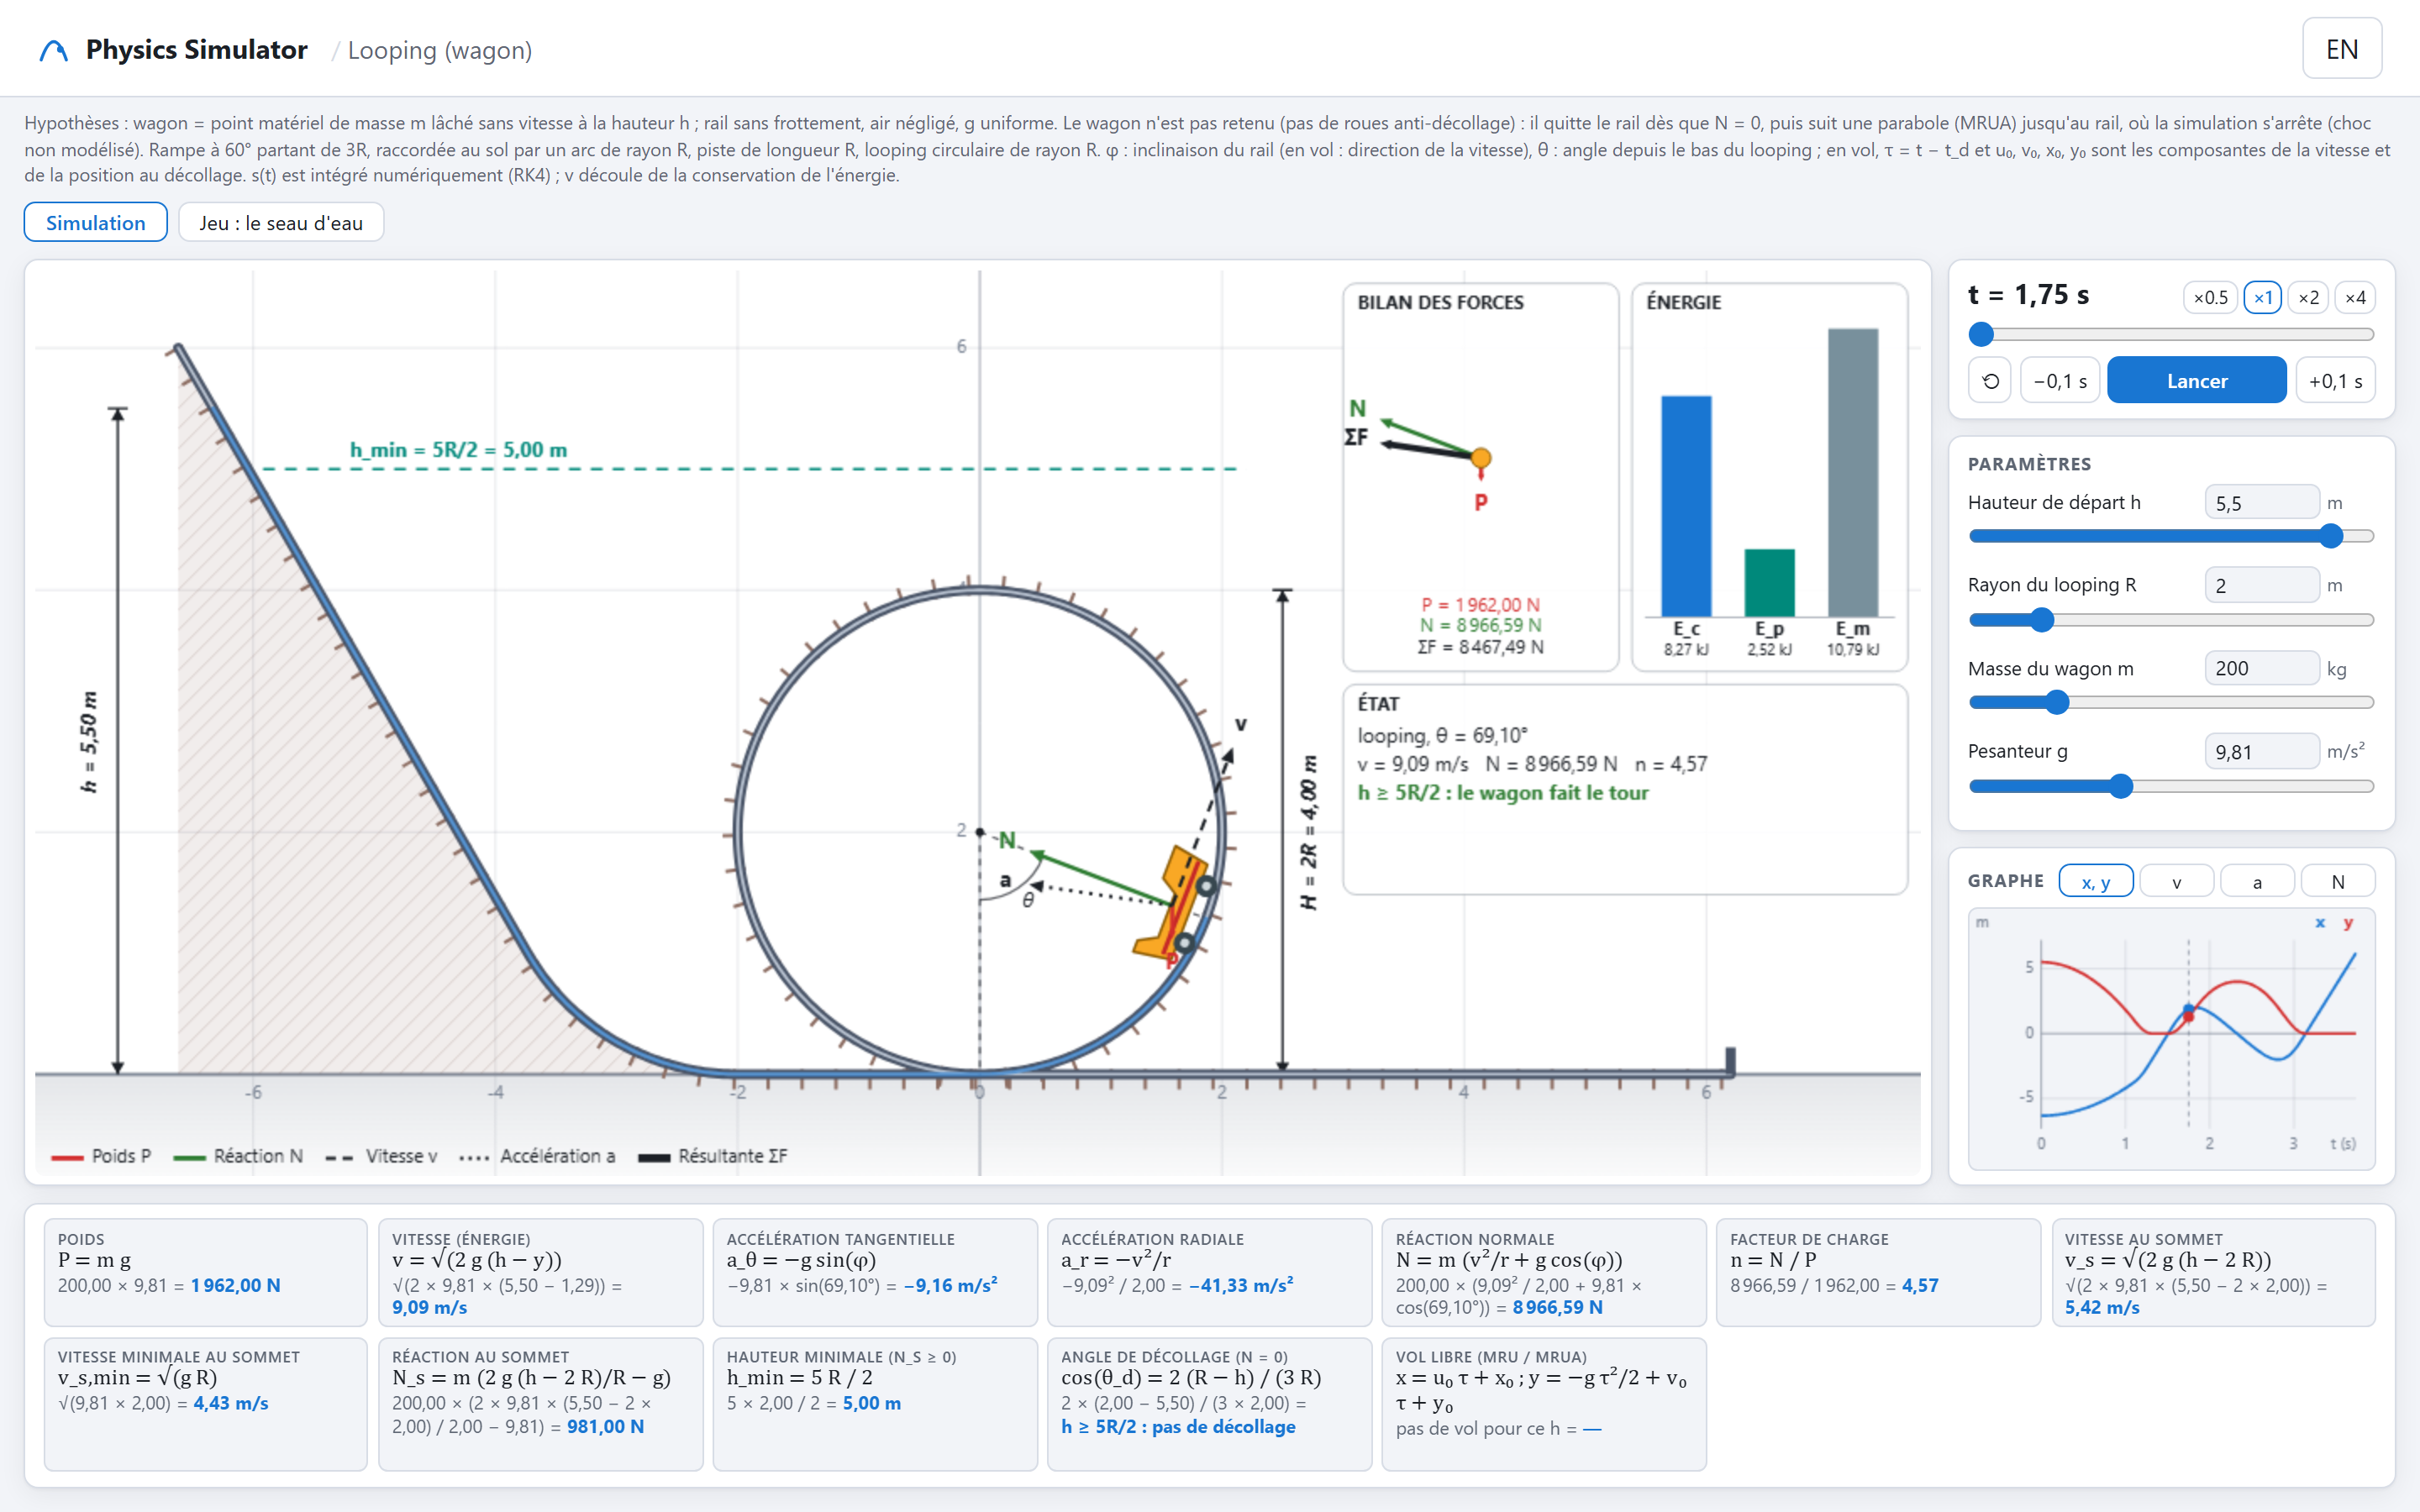
\includegraphics[width=0.78\linewidth]{figures/captures/looping-ecran-complet.png}
  \vfill
  \begin{tabular}{@{}ll@{}}
    Auteur : & Arnaud Gheysens \\
    Promoteur : & [Nom du promoteur] \\
    Lecteurs : & [Noms des lecteurs] \\
  \end{tabular}
  \par\vspace{1cm}
  {\large Mémoire présenté en vue de l'obtention du grade de [master] \par}
  {\large Année académique [2026--2027] \par}
\end{titlepage}

% 00-liminaires.tex — Remerciements, résumé et abstract (hors pagination du corps).

\chapter*{Remerciements}
\addcontentsline{toc}{chapter}{Remerciements}

\begin{arediger}{½ page}
Promoteur, lecteurs, enseignants et étudiants du cours de Physique~1 ayant
participé aux tests, collègues du groupe.
\end{arediger}

\chapter*{Résumé}
\addcontentsline{toc}{chapter}{Résumé}

\begin{arediger}{1 page (résumé + abstract)}
Un paragraphe de 200 à 250 mots, écrit en dernier : problème (difficultés des
étudiants de BAC1 en mécanique : forces, mouvement circulaire, énergie),
démarche (site de simulations interactives développé avec une IA encadrée par
des règles, des tests et des agents ; mode jeu), principaux résultats
(chapitres~\ref{chap:resultats-quantitatifs} et~\ref{chap:resultats-qualitatifs}),
conclusion. Mots-clés : simulation interactive, mécanique, BAC1, ludification,
dynamique basée sur les positions, IA générative.
\end{arediger}

\section*{Abstract}

\begin{arediger}{traduction du résumé}
Version anglaise du résumé, mêmes mots-clés.
\end{arediger}

\tableofcontents
\listoffigures
\listoftables

\cleardoublepage
\pagenumbering{arabic}
% 01-introduction.tex — Introduction générale (≈ 4 pages).

\chapter{Introduction}
\label{chap:introduction}

\section{Contexte}

\begin{arediger}{1 page}
Le cours de Physique~1 en première année d'ingénieur civil : public nombreux,
hétérogène, transition secondaire–université. La mécanique newtonienne
(cinématique, dynamique, énergie, mouvement circulaire) est la première
rencontre avec une physique formalisée. Constat de terrain du professeur :
les étudiants manipulent les formules sans se représenter les forces
(exemple du looping : \enquote{la force centrifuge pousse la bille vers
l'extérieur}). Citer \textcite{hestenes1992fci} et \textcite{hake1998}.
\end{arediger}

\section{Problématique et questions de recherche}

\begin{arediger}{1 page}
Question principale : des simulations interactives conçues pour le cours, qui
montrent en même temps le phénomène, les forces et les formules avec leurs
valeurs numériques, améliorent-elles la compréhension des étudiants de BAC1 ?
Sous-questions : (1) quelles caractéristiques de conception comptent
(représentations liées, contrôle du temps, ludification) ; (2) un enseignant
peut-il produire de telles simulations avec un assistant de programmation
fondé sur l'IA, à un niveau de qualité vérifiable ; (3) quel est l'effet
mesuré sur l'apprentissage et la motivation. Formuler les hypothèses
testées au chapitre~\ref{chap:protocole}.
\end{arediger}

\section{Démarche et contributions}

\begin{arediger}{1 page}
Présenter le site (figure~\ref{fig:intro-accueil}) : quatre à cinq exercices
de mécanique, tous construits sur le même gabarit ; un mode jeu expérimental ;
une méthode de développement assistée par IA reproductible ; un protocole
d'évaluation. Énoncer clairement ce qui est original : la combinaison
formules substituées pas à pas + diagramme des forces + jeu dont la condition
de réussite est la relation du cours (chapitre~\ref{chap:jeu}).
\end{arediger}

\begin{figure}[ht]
  \centering
  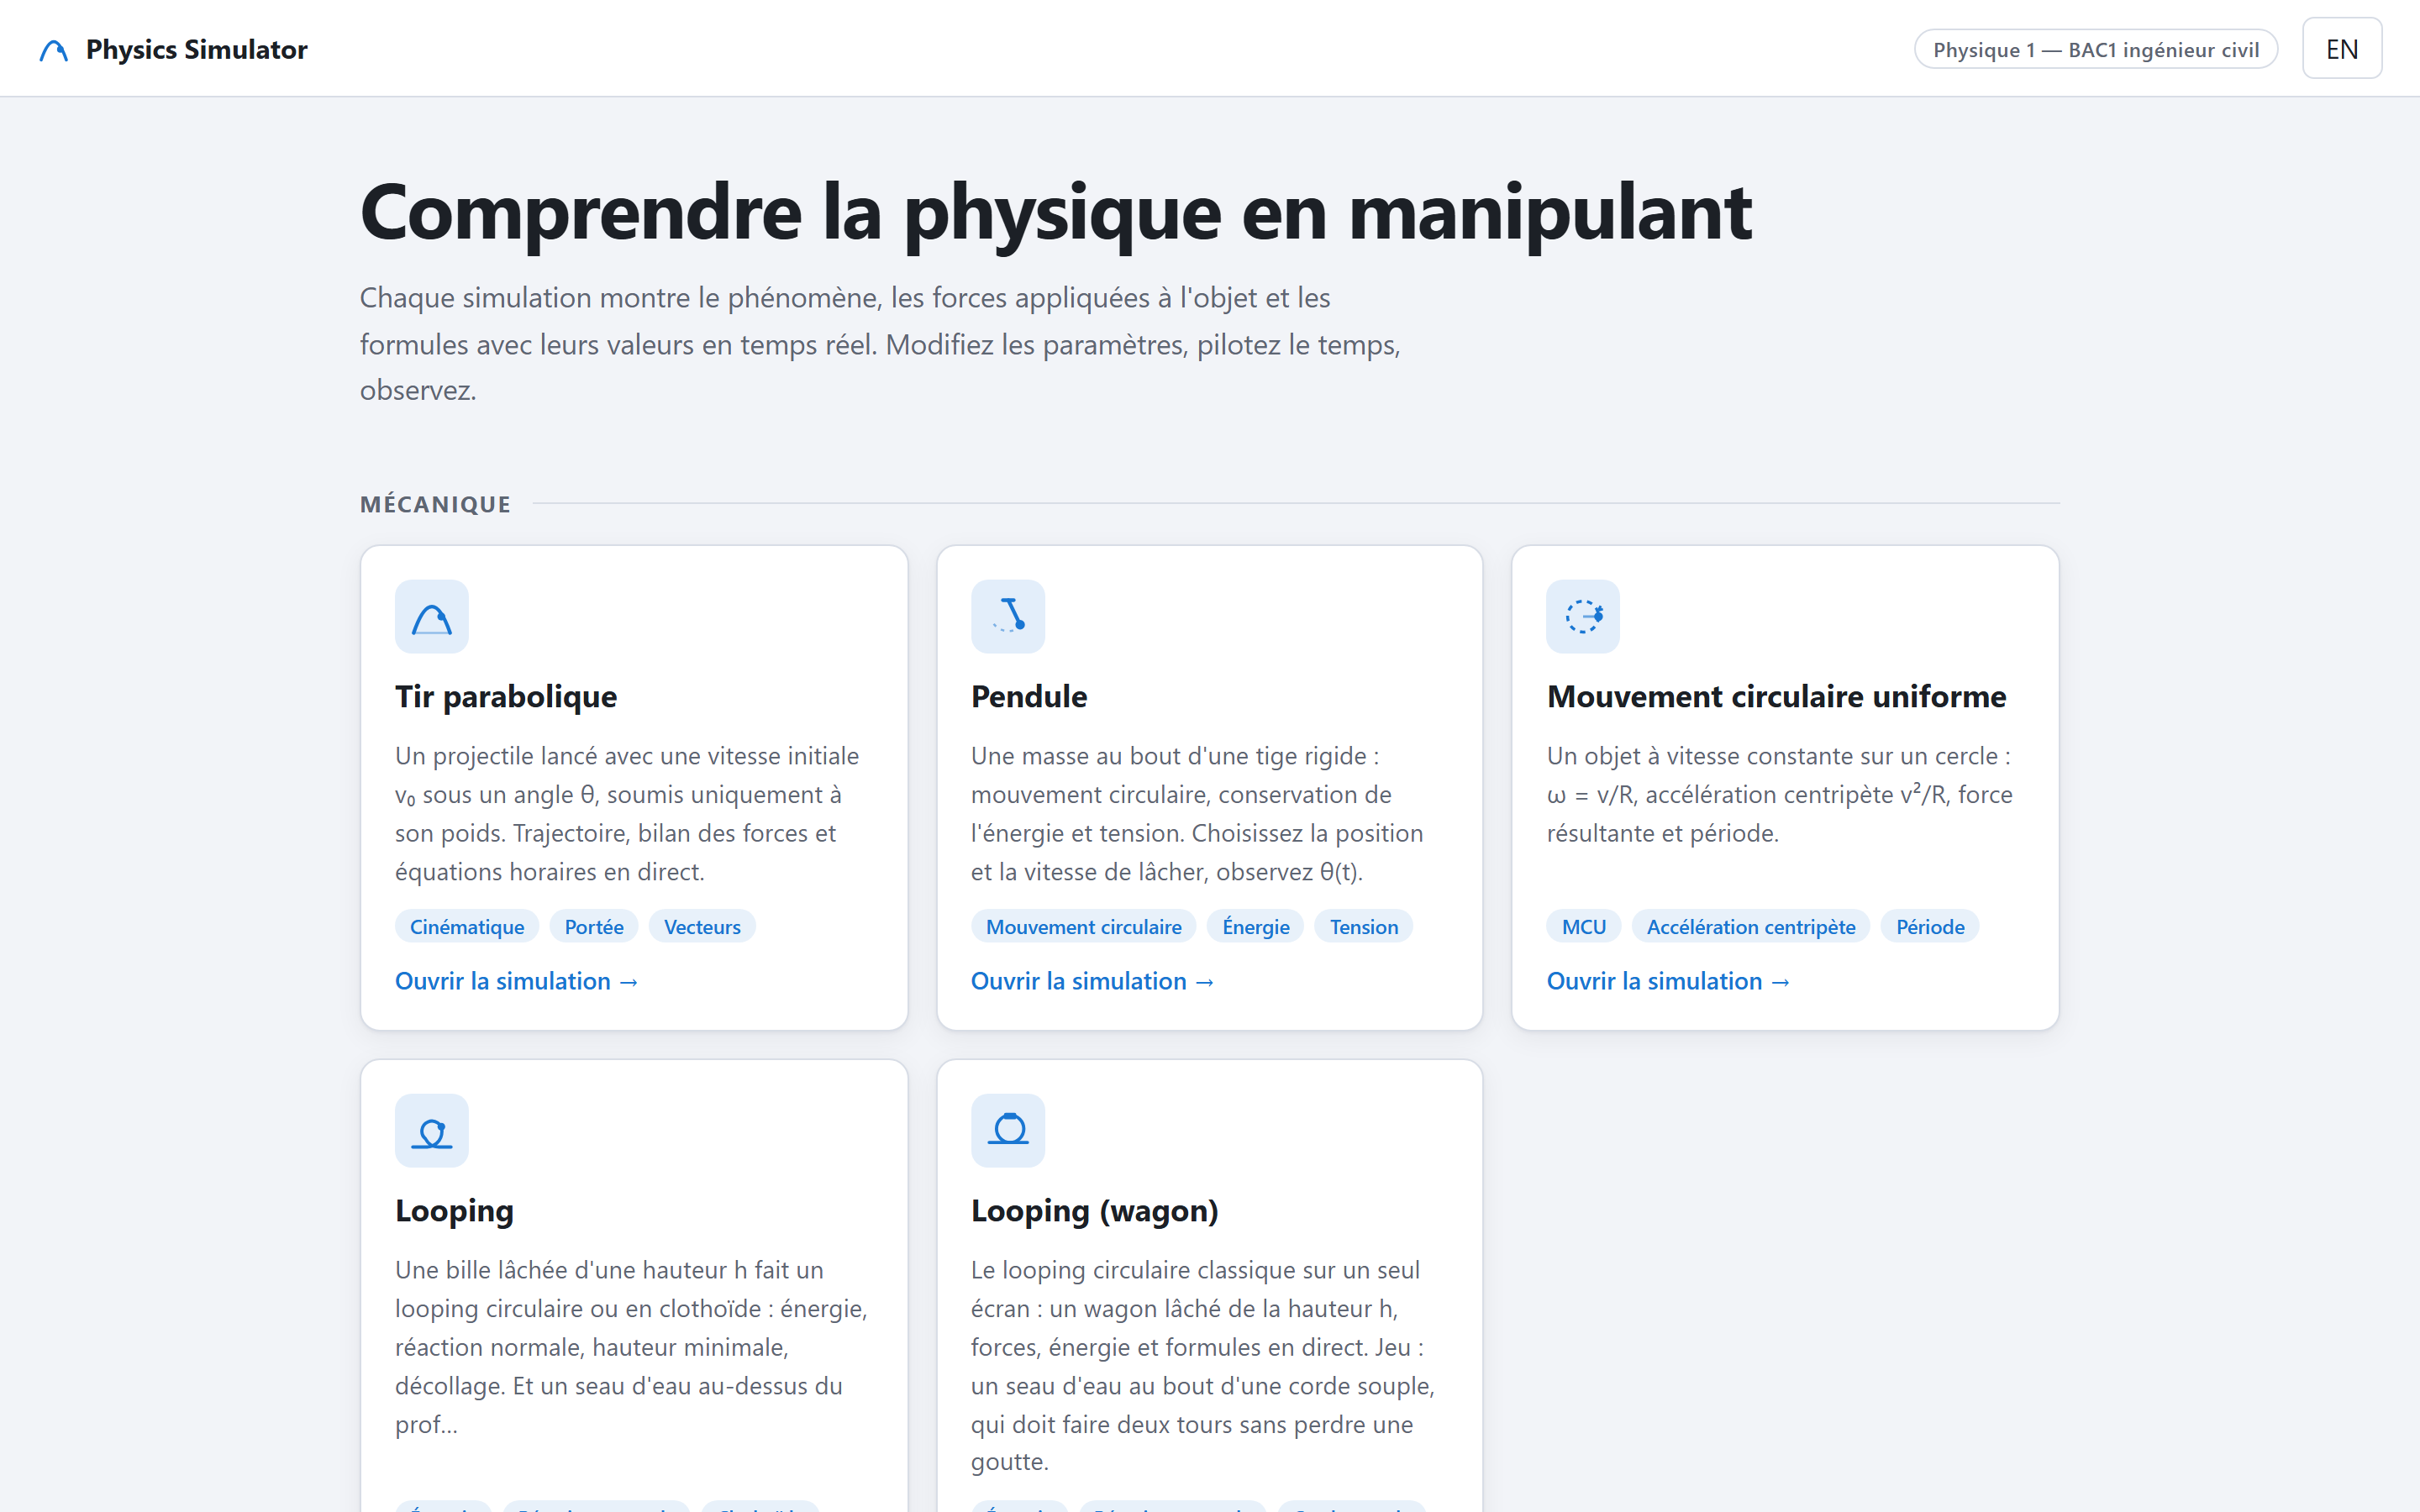
\includegraphics[width=0.85\linewidth]{figures/captures/accueil.png}
  \caption{Page d'accueil du site : un exercice par carte, regroupés par thème.}
  \label{fig:intro-accueil}
\end{figure}

\section{Plan du mémoire}

\begin{arediger}{½ page}
La partie~I fait l'état de l'art (difficultés des étudiants, simulations et
apprentissage, ludification, méthodes numériques, IA pour le développement).
La partie~II décrit la réalisation (cahier des charges et méthodologie,
architecture et exercices, jeu du seau d'eau, validation). La partie~III
présente le protocole, les résultats et leur discussion. Une conclusion
ouvre les perspectives.
\end{arediger}


\part{État de l'art}
% 02-difficultes-mecanique.tex — État de l'art 1/5 : difficultés des étudiants
% en mécanique de première année (≈ 6 pages).

\chapter{Apprendre la mécanique en première année}
\label{chap:difficultes}

\section{La mécanique dans le cursus d'ingénieur civil}

\begin{arediger}{1 page}
Place du cours de Physique~1 (EPL1201) : contenus, formulaire officiel
\parencite{formulaire_epl1201}, notations imposées (\(u_0\), \(v_0\), MRU/MRUA,
\(a_r = -r \omega^2\)). Pourquoi ces notations comptent pour les
simulations (cohérence avec le cours, voir section~\ref{sec:notation}).
\end{arediger}

\section{Conceptions alternatives sur la force et le mouvement}

\begin{arediger}{2 pages}
Littérature sur les préconceptions : force dans le sens du mouvement,
\enquote{force centrifuge}, confusion vitesse/accélération, poids et
réaction normale toujours égaux. Le Force Concept Inventory
\parencite{hestenes1992fci} et ses résultats typiques en début d'université.
Lien direct avec nos exercices : réaction normale variable dans le looping,
tension qui s'annule au sommet.
\end{arediger}

\section{Le mouvement circulaire et la réaction normale}

\begin{arediger}{1,5 page}
Difficultés spécifiques : accélération centripète sans \enquote{force
centripète} supplémentaire, rôle de \(N\) et de \(T\), condition \(N \geq 0\).
Le looping comme situation classique (manuels, attractions ;
\textcite{pendrill2005loops} sur la forme des loopings réels). Présenter la
figure~\ref{fig:etat-normale} : \(N/(m g)\) le long du cercle pour trois
hauteurs.
\end{arediger}

\begin{figure}[ht]
  \centering
  \begin{tikzpicture}
    \begin{axis}[width=0.8\linewidth, height=5.4cm, xmin=0, xmax=360, xtick={0,90,180,270,360},
      xlabel={angle depuis le bas du looping \(\theta\) (°)}, ylabel={\(N / (m g)\)},
      grid=major, grid style={gray!20}, legend pos=north east, legend cell align=left,
      every axis plot/.append style={thick}]
      \addplot[accent] table[x=theta, y=h30, col sep=comma] {figures/donnees/normale_looping.csv};
      \addplot[normale] table[x=theta, y=h25, col sep=comma] {figures/donnees/normale_looping.csv};
      \addplot[poids] table[x=theta, y=h20, col sep=comma] {figures/donnees/normale_looping.csv};
      \addplot[black, dashed, thin] coordinates {(0,0) (360,0)};
      \legend{\(h = 3R\), \(h = 5R/2\) (limite), \(h = 2R\)}
    \end{axis}
  \end{tikzpicture}
  \caption{Réaction normale réduite \(N/(m g) = 2 (h - y)/R + \cos(\theta)\) le long
    du looping, avec \(y = R (1 - \cos(\theta))\). Pour \(h = 5R/2\), \(N\) s'annule
    exactement au sommet ; pour \(h = 2R\), elle devient négative : le wagon quitte
    le rail. Données générées par le code de l'application (\fichier{outils/donnees.mjs}).}
  \label{fig:etat-normale}
\end{figure}

\section{L'énergie mécanique comme outil de raisonnement}

\begin{arediger}{1,5 page}
Conservation de l'énergie, choix d'une référence, passage énergie
\(\rightarrow\) vitesse \(\rightarrow\) force. Difficulté à combiner deux
principes (énergie et deuxième loi de Newton) dans un même problème : c'est
exactement ce qu'exige la condition \(h_{\min} = 5R/2\).
\end{arediger}

% 03-simulations-apprentissage.tex — État de l'art 2/5 : simulations
% interactives et apprentissage (≈ 7 pages).

\chapter{Simulations interactives et apprentissage}
\label{chap:simulations}

\section{Pédagogies actives en physique}

\begin{arediger}{1,5 page}
Engagement interactif contre enseignement traditionnel : gains normalisés
\parencite{hake1998}, méta-analyse de l'apprentissage actif \parencite{freeman2014}.
Ce qu'une simulation peut apporter dans un amphithéâtre ou en travail
autonome.
\end{arediger}

\section{Les simulations de physique : PhET et au-delà}

\begin{arediger}{2 pages}
PhET \parencite{wieman2008phet, adams2008phet} : principes de conception
(rétroaction immédiate, représentations multiples, exploration guidée),
études d'engagement. Comparaison laboratoire réel / virtuel
\parencite{finkelstein2005}. Tableau comparatif d'outils existants (PhET,
myPhysicsLab, GeoGebra, Algodoo…) : contrôle du temps, affichage des
forces, formules substituées, adaptation au cours. Montrer ce qui manque
pour un cours précis de BAC1.
\end{arediger}

\section{Apprentissage par découverte et guidage}

\begin{arediger}{1,5 page}
\textcite{dejong1998} : la découverte avec simulation n'est efficace qu'avec
du guidage (hypothèses, variables, consignes). Conséquence pour nos pages :
hypothèses affichées, verdict explicite (\enquote{le wagon fait le tour} /
\enquote{décollage à \(\theta_d\)}), défis du mode jeu.
\end{arediger}

\section{Charge cognitive et représentations multiples}

\begin{arediger}{2 pages}
Théorie de la charge cognitive \parencite{sweller1988} et principes du
multimédia \parencite{mayer2009} : contiguïté spatiale et temporelle,
signalement, cohérence. Justifie nos choix : formules à côté de la scène,
valeurs numériques substituées, code couleur constant des vecteurs, tout sur
un seul écran (section~\ref{sec:exercice-wagon}).
\end{arediger}

% 04-ludification.tex — État de l'art 3/5 : ludification et jeux sérieux (≈ 4 pages).

\chapter{Ludification et jeux sérieux}
\label{chap:ludification}

\section{Définitions}

\begin{arediger}{1 page}
Ludification (éléments de jeu dans un contexte non ludique,
\cite{deterding2011}) contre jeu sérieux ; mécaniques usuelles : objectifs,
paliers, rétroaction, défi adapté.
\end{arediger}

\section{Effets sur la motivation et l'apprentissage}

\begin{arediger}{2 pages}
Résultats contrastés de la littérature : motivation à court terme, risque de
\enquote{chasse au curseur} sans compréhension. Condition d'efficacité : la
règle du jeu doit être la relation physique elle-même. C'est le principe de
notre mode jeu : gagner exige \(v_0^2 \geq 5 g R\) et \(m (v_0^2/R + g) \leq T_{\max}\).
\end{arediger}

\section{Réalisme et sobriété}

\begin{arediger}{1 page}
Arbitrage entre animation spectaculaire et sobriété : la première version du
jeu (personnage animé, confettis) a été remplacée par une version sobre
(\enquote{réussi} / \enquote{raté}) mais physiquement plus réaliste (corde
souple, eau en particules). Discuter ce choix à la lumière du principe de
cohérence \parencite{mayer2009}.
\end{arediger}

% 05-methodes-numeriques.tex — État de l'art 4/5 : méthodes numériques pour
% la simulation physique interactive (≈ 4 pages).

\chapter{Méthodes numériques pour la simulation interactive}
\label{chap:methodes}

\section{Intégrer les équations du mouvement}

\begin{arediger}{1,5 page}
Euler explicite, Euler semi-implicite, Verlet \parencite{verlet1967},
Runge--Kutta d'ordre~4 \parencite{butcher2016} ; précision, stabilité,
conservation de l'énergie \parencite{hairer2006}. Justifier RK4 pour le
mouvement le long du rail (une seule équation \(\ddot{s} = -g \sin(\varphi)\))
et les formes exactes partout où elles existent (parabole, énergie).
\end{arediger}

\section{Dynamique basée sur les positions}

\begin{arediger}{1,5 page}
Principe de la dynamique basée sur les positions \parencite{muller2007pbd,
bender2014survey}, sa version étendue XPBD \parencite{macklin2016xpbd} et
l'approche à petits pas \parencite{macklin2019smallsteps} ; précurseur dans le
jeu vidéo \parencite{jakobsen2001}. Cordes, cheveux et tiges : projection
\enquote{follow-the-leader} \parencite{muller2012ftl} et solveur direct pour
chaînes \parencite{deul2018direct}. Le chapitre~\ref{chap:jeu} applique ces
méthodes.
\end{arediger}

\section{Fluides particulaires}

\begin{arediger}{1 page}
SPH \parencite{monaghan1992sph} et fluides basés sur les positions
\parencite{macklin2013pbf}. Pourquoi nous nous limitons à dix particules sans
pression ni viscosité : on veut voir \emph{quand} l'eau sort du seau, pas
comment elle s'écoule.
\end{arediger}

% 06-ia-developpement.tex — État de l'art 5/5 : IA générative et
% développement de ressources éducatives (≈ 3 pages).

\chapter{IA générative et développement de ressources éducatives}
\label{chap:ia}

\section{Les assistants de programmation}

\begin{arediger}{1,5 page}
Modèles de langage entraînés sur du code \parencite{chen2021codex} ;
assistants agentiques capables de lire un dépôt, exécuter des tests et
déléguer à des sous-agents. Forces (vitesse, couverture) et limites
(hallucinations, choix implicites, vérification nécessaire).
\end{arediger}

\section{IA et éducation}

\begin{arediger}{1,5 page}
Opportunités et risques pour l'enseignement \parencite{kasneci2023}. Position de
ce travail : l'IA n'est pas utilisée par les étudiants mais par
l'enseignant pour produire des ressources, sous contrôle de règles écrites,
de tests automatiques et de vérifications physiques indépendantes
(section~\ref{sec:methodologie}).
\end{arediger}


\part{Réalisation}
% 07-cahier-des-charges.tex — Réalisation 1/4 : exigences pédagogiques et
% techniques, puis méthodologie de développement assistée par IA (≈ 8 pages,
% dont la méthodologie déjà rédigée dans sections/methodologie.tex).

\chapter{Cahier des charges et méthode de travail}
\label{chap:cahier}

\section{Exigences pédagogiques}

\begin{arediger}{1 page}
Traduire l'état de l'art en exigences vérifiables : chaque page montre le
phénomène, \emph{toutes} les forces avec un code couleur constant (poids
rouge, réaction verte, tension violette, vitesse en tirets, accélération en
pointillés, résultante épaisse), un diagramme des forces toujours visible,
les formules sous trois formes (symbolique, valeurs substituées, résultat
avec unité), les hypothèses écrites, des graphes temporels synchronisés et
un contrôle complet du temps. Notations du formulaire du cours.
\end{arediger}

\section{Exigences techniques}

\begin{arediger}{1 page}
Site statique (HTML, CSS, JavaScript sans bibliothèque) qui fonctionne par
double-clic (\fichier{file://}), sur PC, tablette et téléphone ; physique
isolée dans un fichier par exercice, facile à auditer ; mode jeu supprimable
en quatre étapes. Expliquer pourquoi chaque contrainte a été choisie.
\end{arediger}

\input{sections/methodologie}

% 08-architecture-et-exercices.tex — Réalisation 2/4 : architecture du site et
% exercices, avec l'exemple détaillé du looping avec wagon (≈ 8 pages).

\chapter{Architecture du site et exercices}
\label{chap:architecture}

\section{Organisation du code}

\begin{arediger}{1,5 page}
Un dossier par thème, un sous-dossier par exercice contenant exactement
\fichier{index.html}, \fichier{calcul.js} (physique pure, testable sous Node),
\fichier{main.js} (affichage et interactions) et éventuellement
\fichier{game.js}. Code visuel partagé (\fichier{canvas\_draw.js},
\fichier{graph\_plot.js}) mais jamais la physique. Scripts classiques exposant
un seul objet global, condition pour fonctionner en \fichier{file://}.
Schéma TikZ des dépendances entre fichiers.
\end{arediger}

\section{Gabarit commun d'une page}

\begin{arediger}{1,5 page}
Scène (canevas redessiné à chaque image), panneau de transport (lecture,
pause, vitesse \(\times 0{,}5\) à \(\times 4\), curseur temporel), paramètres
(curseur + champ numérique), formules, graphes. Bilingue FR/EN. Présenter
brièvement les exercices existants (tir parabolique, pendule, MCU, looping).
\end{arediger}

\section{Exemple détaillé : le looping avec wagon}
\label{sec:exercice-wagon}

La dernière version du looping a été conçue pour tenir sur un seul écran
(figure~\ref{fig:wagon-ecran}). Le rail est entièrement proportionnel au rayon
\(R\) du looping : rampe à \ang{60} partant de \(3R\), raccord circulaire de rayon
\(R\), piste de longueur \(R\), cercle de rayon \(R\). La vue est donc un cadre
fixe exprimé en unités de \(R\) : changer \(R\) ne change que l'échelle de la
grille, l'image ne bouge jamais et l'étudiant ne peut ni zoomer ni se déplacer.
Cette propriété permet de placer dans l'espace libre du canevas le diagramme des
forces, les barres d'énergie \(E_c\), \(E_p\), \(E_m\) et un état en direct
(position sur le rail, \(v\), \(N\), facteur de charge \(n\), verdict).

\begin{figure}[ht]
  \centering
  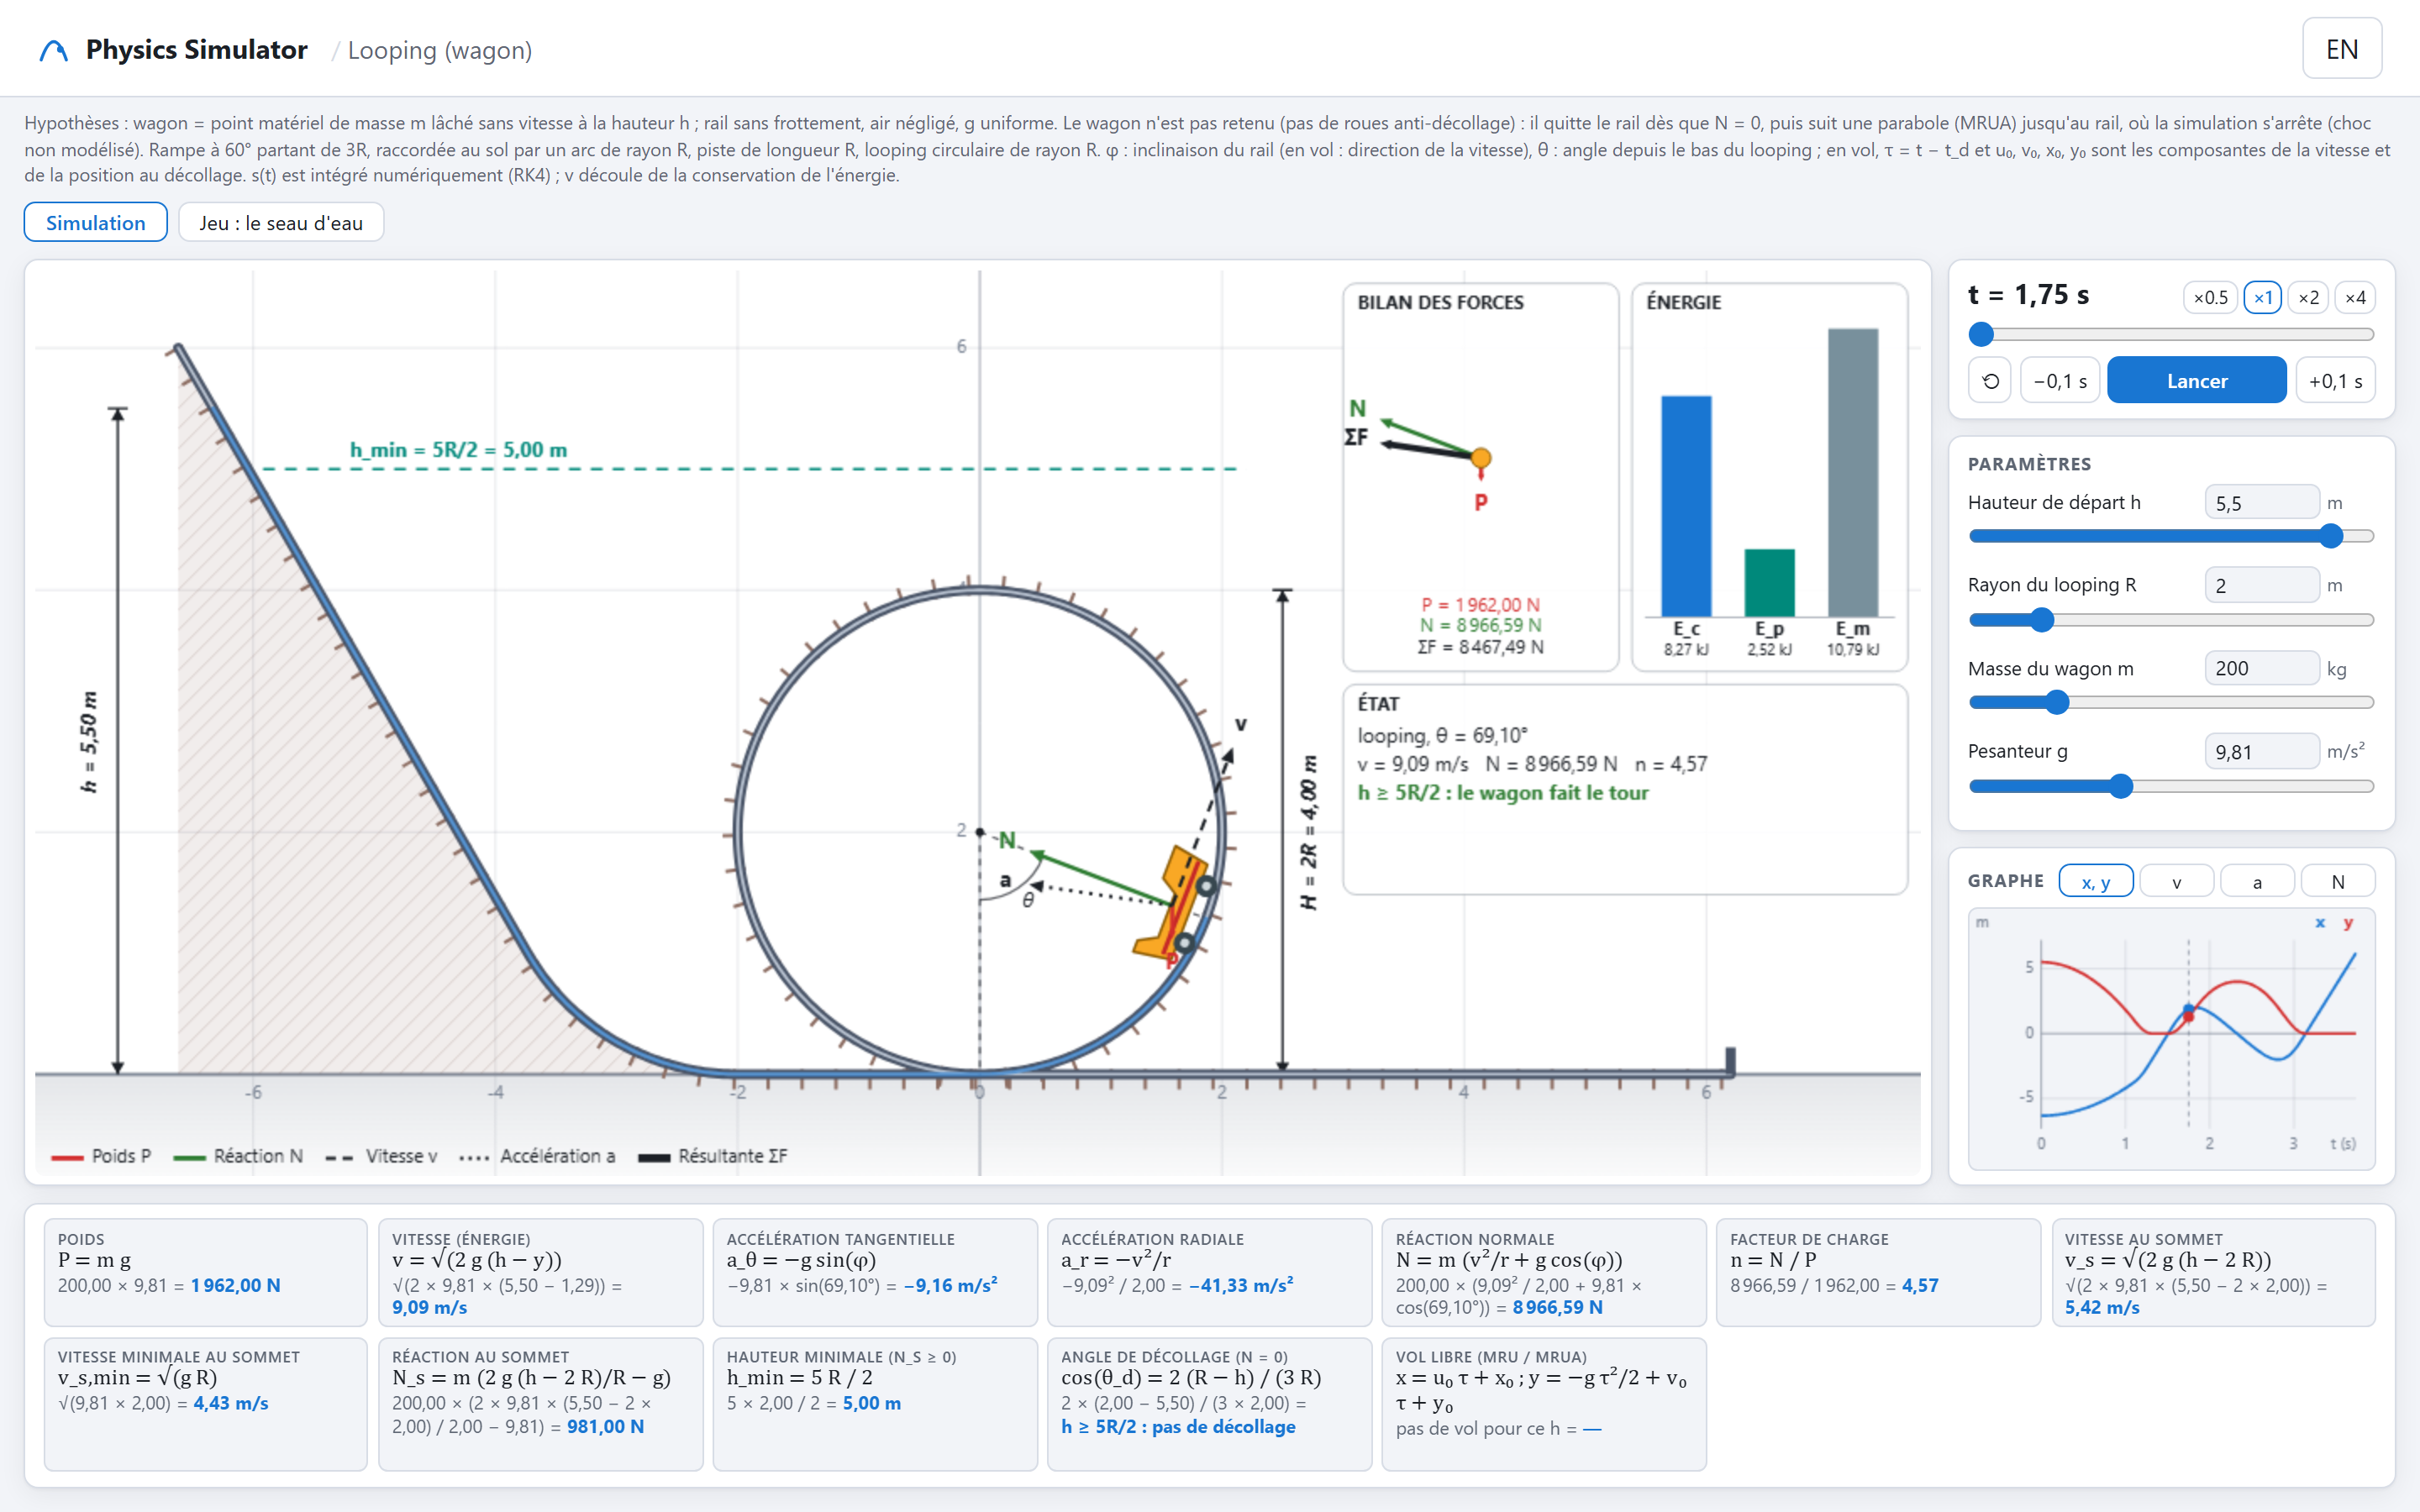
\includegraphics[width=\linewidth]{figures/captures/looping-ecran-complet.png}
  \caption{Exercice du looping avec wagon sur un écran de \(1440 \times 900\)
    pixels : scène avec vecteurs \(P\), \(N\), \(v\), \(a\), diagramme des forces,
    énergies et état dans l'espace libre du canevas ; transport, paramètres et
    graphe à droite ; douze formules substituées en bas.}
  \label{fig:wagon-ecran}
\end{figure}

\begin{arediger}{3 pages}
Rédiger : (1) le modèle (point matériel, rail sans frottement, wagon non
retenu) et les équations affichées : \(v = \sqrt{2 g (h - y)}\),
\(a_\theta = -g \sin(\varphi)\), \(a_r = -v^2/r\),
\(N = m (v^2/r + g \cos(\varphi))\), \(n = N/P\),
\(v_s = \sqrt{2 g (h - 2R)} \geq \sqrt{g R}\), \(h_{\min} = 5R/2\),
\(\cos(\theta_d) = 2 (R - h)/(3 R)\), vol libre en MRU/MRUA ; (2) les trois
régimes (le wagon fait le tour, décolle, fait demi-tour) avec la
figure~\ref{fig:wagon-decollage} ; (3) l'intégration RK4 de \(s(t)\) et le
calcul exact de \(v\) par l'énergie ; (4) les choix d'interface justifiés par
le chapitre~\ref{chap:simulations} (un seul écran, contiguïté, couleurs).
\end{arediger}

\begin{figure}[ht]
  \centering
  \begin{subfigure}[b]{0.70\linewidth}
    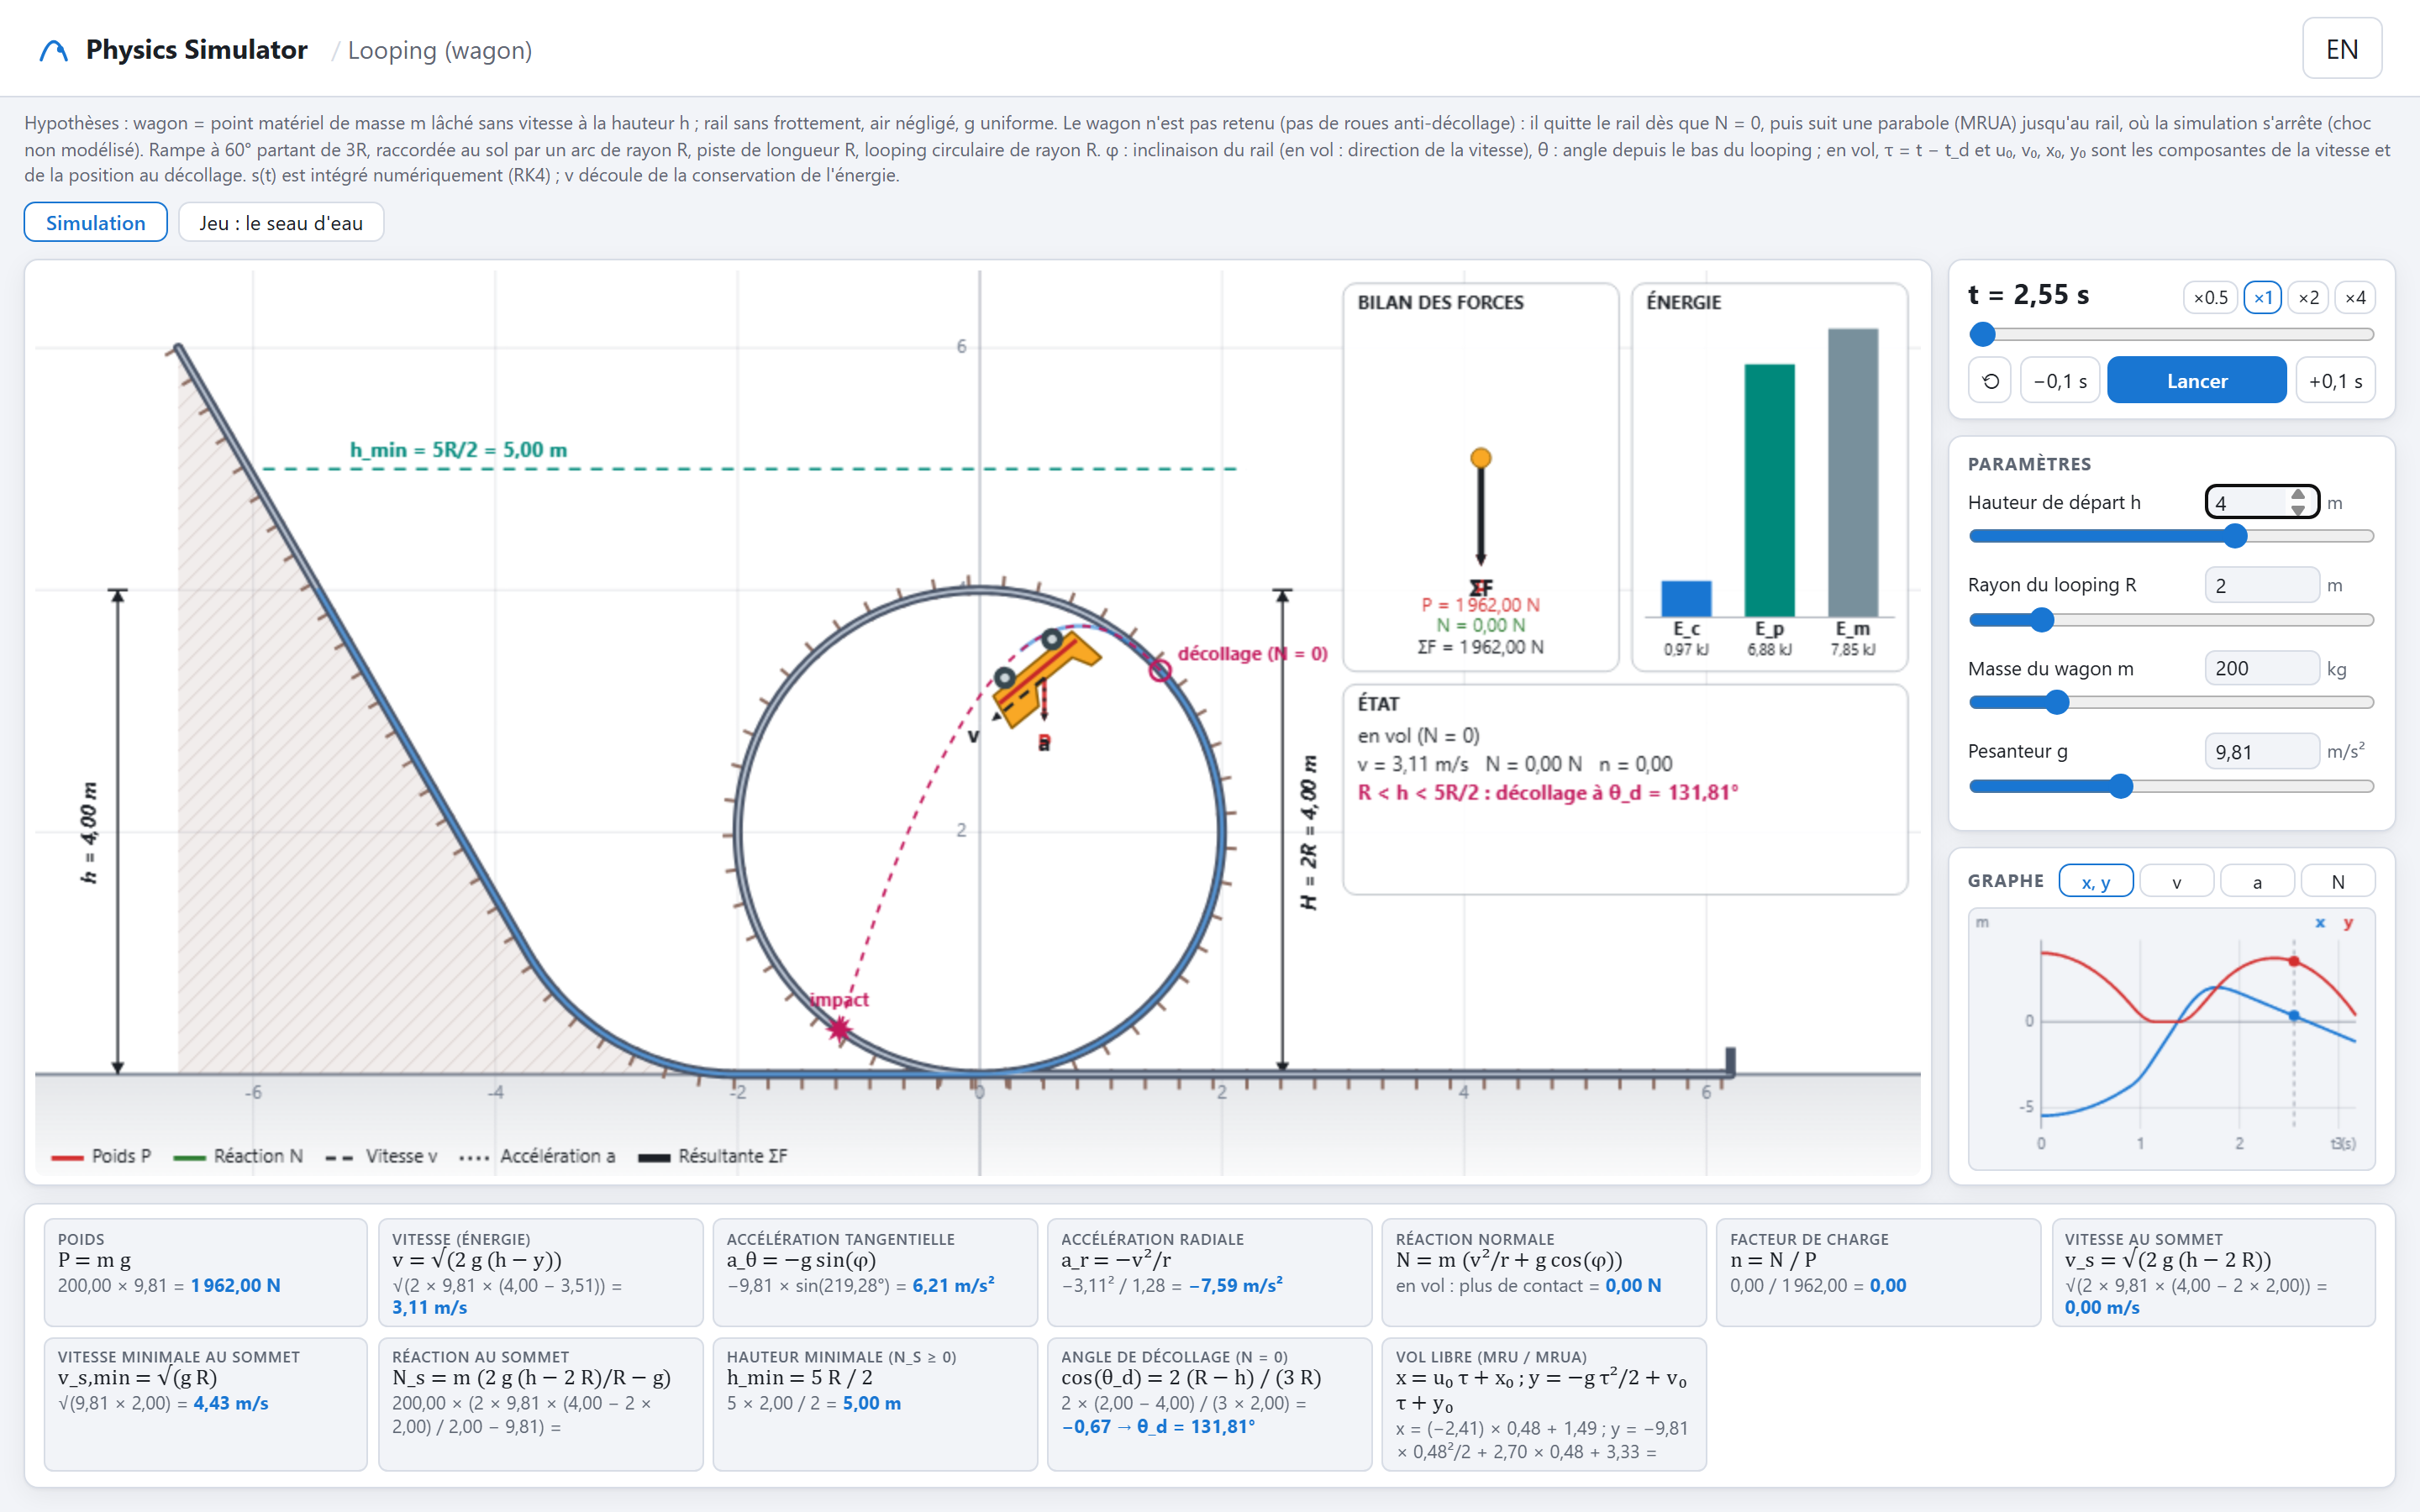
\includegraphics[width=\linewidth]{figures/captures/looping-decollage.png}
    \caption{\(h = 4\) m pour \(R = 2\) m : décollage prévu à
      \(\theta_d = \ang{131,81}\), parabole en tirets jusqu'à l'impact.}
  \end{subfigure}\hfill
  \begin{subfigure}[b]{0.27\linewidth}
    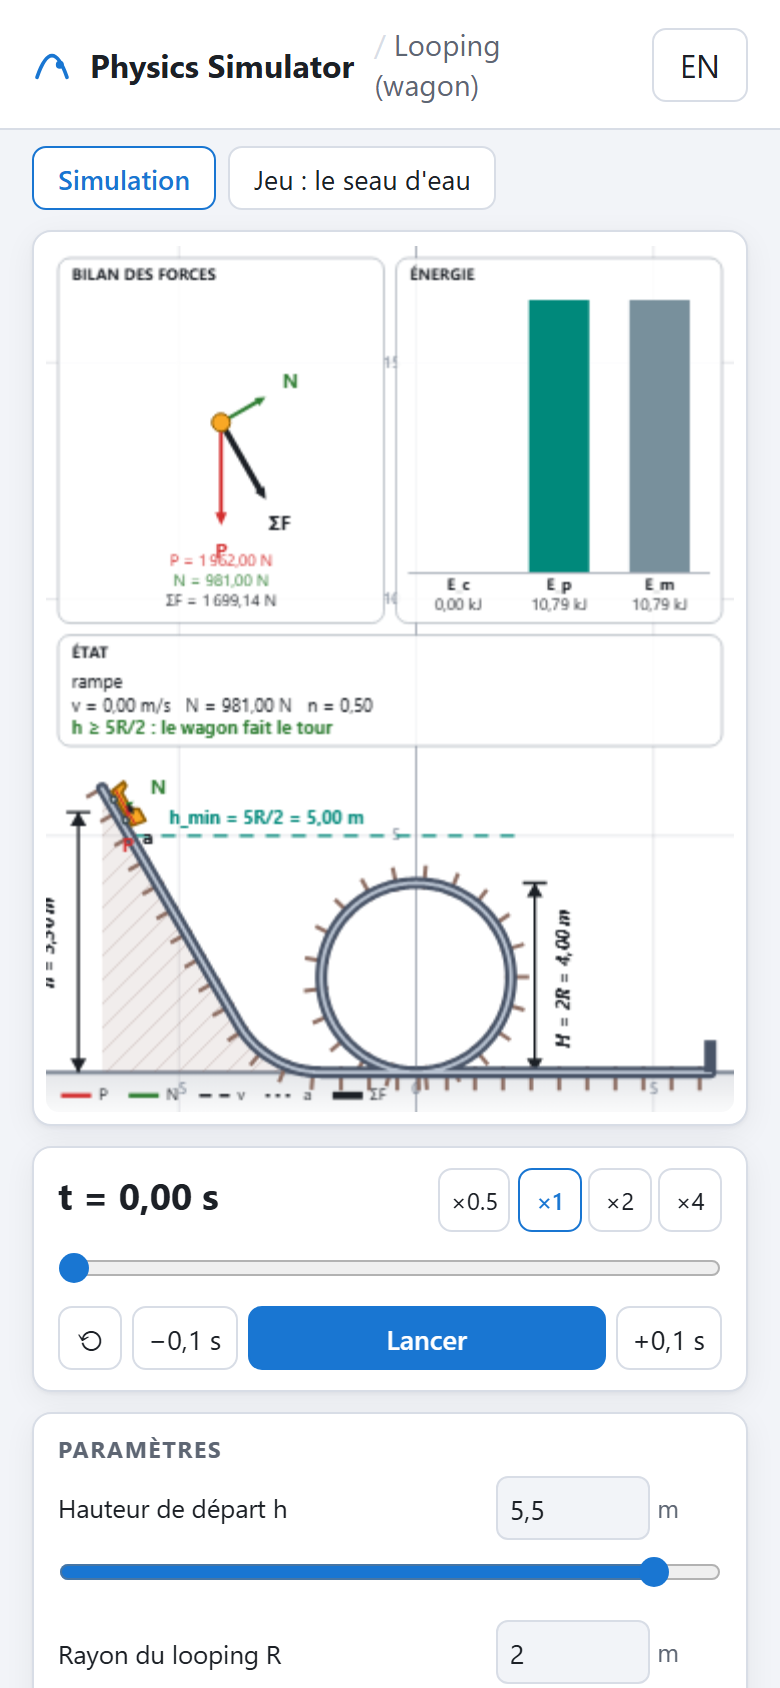
\includegraphics[width=\linewidth]{figures/captures/looping-telephone.png}
    \caption{Même page sur téléphone : bandeau d'informations au-dessus du rail.}
  \end{subfigure}
  \caption{Cas du décollage (\(R < h < 5R/2\)) et adaptation à un écran étroit.}
  \label{fig:wagon-decollage}
\end{figure}

\section{Le mode jeu : principe commun}

\begin{arediger}{1 page}
Règles communes à tous les jeux : une seule grandeur libre, situation tirée au
hasard mais \emph{prouvablement soluble} (génération constructive autour d'une
solution de référence, vérificateur pur, tirage par rejet, cas de repli),
paliers 1, 5, 10, 20, 40, 70, 100, formules et graphes cachés, mise en page
identique au mode normal. Le jeu du looping est détaillé au chapitre suivant.
\end{arediger}

% 09-jeu-seau.tex — Réalisation 3/4 : le jeu du seau d'eau (≈ 5 pages, rédigé).
% Implémentation : src/mechanics/loop-wagon/game.js. Les chiffres cités sont
% mesurés sur ce code (outils/donnees.mjs, tests unitaires game.test.js).

\chapter{Le jeu du seau d'eau : une corde qui plie et de l'eau en particules}
\label{chap:jeu}

\section{Principe du jeu et lien avec le looping}

Le mode jeu de l'exercice du looping remplace le wagon par une expérience que
tout le monde a vue, ou faite : faire tourner un seau d'eau à bout de bras sans
se mouiller. Une barre légère tourne librement autour d'un pivot fixe ; une corde
souple est attachée à son extrémité et porte un seau ouvert contenant dix gouttes
d'eau. Au départ, tout pend au repos ; une main balance le seau, puis le lance
(section~\ref{sec:jeu-main}) de sorte qu'il passe au point bas avec la vitesse
\(v_0\). Le défi est réussi si le seau fait deux tours sans
perdre une seule goutte et sans casser la corde ; sinon il est raté. Chaque défi
impose le lieu (Lune, Mars, Vénus, Terre, donc \(g\)) et toutes les grandeurs
sauf une, que l'étudiant règle : la vitesse \(v_0\), la longueur de corde \(L\)
ou la masse \(m\) du seau rempli.

Tant que la corde est tendue, barre, corde et seau restent alignés et forment
un pendule de rayon \(R = L_b + L + d\), où \(L_b = \SI{0,50}{m}\) est la longueur
de la barre et \(d = \SI{0,19}{m}\) la distance de l'anse au centre de masse du
seau. La conservation de l'énergie donne \(v^2 = v_0^2 - 2 g R (1 - \cos(\theta))\),
\(\theta\) étant l'angle depuis le point bas, et la deuxième loi de Newton selon
la direction radiale donne la tension
\begin{equation}
  T = m \left(\frac{v^2}{R} + g \cos(\theta)\right)
    = m \left(\frac{v_0^2}{R} + g \, (3 \cos(\theta) - 2)\right).
  \label{eq:jeu-tension}
\end{equation}
C'est exactement la réaction normale du wagon, \(N = m (v^2/r + g \cos(\varphi))\),
avec \(v_0^2 = 2 g h\) (tableau~\ref{tab:jeu-analogie}). Pourquoi l'eau reste-t-elle
dans le seau ? Seuls le poids \(\vect{P}\) et la tension \(\vect{T}\) agissent sur
le seau, donc \(\vect{a} = \vect{g} + \vect{T}/m\). Une goutte libre a pour
accélération \(\vect{g}\) ; relativement au seau, elle accélère donc de
\(-\vect{T}/m\), c'est-à-dire vers le fond du seau tant que \(T > 0\). L'eau
reste dans le seau si et seulement si la corde reste tendue, et la condition la
plus sévère est au sommet : \(T_s = m (v_0^2/R - 5 g) \geq 0\), soit
\(v_0^2 \geq 5 g R\). La corde résiste si la tension maximale, au point bas, ne
dépasse pas la tension de rupture : \(m (v_0^2/R + g) \leq T_{\max}\).

\begin{table}[ht]
  \centering\small
  \begin{tabular}{@{}lll@{}}
    \toprule
    & Wagon sur le looping & Seau au bout de la corde \\
    \midrule
    Force de contact & réaction normale \(N\) & tension \(T\) \\
    Énergie disponible & \(v_{\text{bas}}^2 = 2 g h\) & \(v_0^2\) \\
    Contact perdu si & \(N < 0\) : décollage du rail & \(T = 0\) : corde molle, l'eau tombe \\
    Condition au sommet & \(h \geq 5R/2\) & \(v_0^2 \geq 5 g R\) \\
    Limite supplémentaire & --- & \(m (v_0^2/R + g) \leq T_{\max}\) \\
    \bottomrule
  \end{tabular}
  \caption{Le jeu reprend la physique de l'exercice : la condition de réussite est
    la relation du cours, pas un réglage à l'aveugle.}
  \label{tab:jeu-analogie}
\end{table}

\paragraph{Pourquoi une barre libre et non un moteur ?} Une barre entraînée à
vitesse angulaire \(\omega\) constante donne un comportement chaotique. Dans le
référentiel tournant, le seau pendu à une corde de longueur \(\ell\) fixée à la
distance \(a\) du pivot est un pendule centrifuge (\(\Omega = \omega \sqrt{a/\ell}\))
forcé une fois par tour par la pesanteur ; l'amplitude forcée, environ
\(g / (\omega^2 |a - \ell|)\), est de l'ordre de \SI{1}{rad} près du seuil. Une barre
légère sur un pivot sans frottement ne transmet au contraire aucun couple : la
corde tendue s'aligne sur elle et la relation~\eqref{eq:jeu-tension} vaut.

\section{Un modèle discret : une chaîne de points}

Le système est représenté par une chaîne de treize points matériels
(figure~\ref{fig:jeu-schema}). Le pivot \(P_0\) est fixe. L'extrémité de la barre
\(P_1\) porte la masse effective \(m_b/3\), qui reproduit le moment d'inertie
\(I = m_b L_b^2/3\) d'une barre homogène de masse \(m_b = \SI{0,3}{kg}\) ; on y applique
le poids \(m_b g/2\), pour que le couple du poids, \(m_b g \, (L_b/2) \sin(\alpha)\), soit
exact. La corde
est découpée en dix maillons de longueur \(\ell = L/10\) séparés par les nœuds
\(P_2\) à \(P_{11}\), chacun de masse \(\mu \ell\) avec une masse linéique
\(\mu = \SI{0,15}{kg/m}\) ; \(P_{11}\) est l'anse du seau et \(P_{12}\) son centre
de masse, de masse \(m\). Deux liaisons sont rigides dans les deux sens : la barre
\(|P_1 - P_0| = L_b\) et le seau \(|P_{12} - P_{11}| = d\), qui fait du seau un
solide articulé à son anse. Les dix maillons de corde sont \emph{unilatéraux} :
\(|P_{i+1} - P_i| \leq \ell\). Un maillon peut raccourcir, jamais s'allonger, et
aucun angle n'est imposé entre deux maillons. C'est ce qui rend la corde
pliable : tendue, elle est droite ; détendue, elle se courbe et ne pousse pas le
seau.

\begin{figure}[ht]
  \centering
  \begin{tikzpicture}[x=1cm, y=1cm, >={Stealth[length=2mm]},
      noeud/.style={circle, fill=corde, inner sep=1.3pt},
      etiquette/.style={font=\scriptsize, align=center}]
    \fill[metal!60] (-0.25,-0.35) -- (0.25,-0.35) -- (0,0) -- cycle;
    \draw[line width=3pt, metal] (0,0) -- (2.2,0);
    \fill[black] (0,0) circle (3pt);
    \node[etiquette, above] at (0,0.1) {\(P_0\)\\pivot fixe};
    \node[etiquette, below] at (1.1,-0.15) {barre rigide \(L_b\)};
    \foreach \k in {0,...,10} {
      \coordinate (c\k) at ({2.2 + 0.5*\k}, {-0.55*sin(18*\k)});
    }
    \draw[corde, line width=1.4pt] (c0) \foreach \k in {1,...,10} { -- (c\k) };
    \foreach \k in {1,...,9} { \node[noeud] at (c\k) {}; }
    \fill[metal] (c0) circle (2.4pt);
    \node[etiquette, above] at (c0) {\(P_1\)\\\(m_b/3\)};
    \node[etiquette, below] at (c5) {\(P_2 \ldots P_{10}\) : nœuds de corde \(\mu \ell\)\\maillons \(|P_{i+1} - P_i| \leq \ell\)};
    \draw[metal, line width=1.2pt, fill=metal!15] (7.6,-0.65) -- (8.85,-0.58) -- (8.85,0.58) -- (7.6,0.65) -- cycle;
    \draw[thin] (7.6,0.65) .. controls (7.0,0.45) and (7.0,-0.45) .. (7.6,-0.65);
    \foreach \x/\y in {8.68/-0.42, 8.68/-0.14, 8.68/0.14, 8.68/0.42, 8.44/-0.28, 8.44/0, 8.44/0.28, 8.2/-0.14, 8.2/0.14, 7.96/0} {
      \fill[eau] (\x,\y) circle (0.12);
    }
    \fill[black] (7.2,0) circle (2pt);
    \node[etiquette, above left] at (7.2,0.05) {\(P_{11}\)\\anse};
    \fill[poids] (8.4,0) circle (2pt);
    \node[etiquette, right] at (8.95,0.25) {\(P_{12}\) : centre\\de masse, \(m\)};
    \draw[->, accent, thick] (7.2,0) -- (7.2,-1.1) node[below, etiquette] {\(\vect{n}\)};
    \draw[->, accent, thick] (8.4,-0.95) -- (9.3,-0.95) node[right, etiquette] {\(\vect{e}\)};
    \draw[|-|, thin] (7.2,1.0) -- node[above, etiquette] {\(u_{\text{bord}}\)} (7.6,1.0);
    \draw[|-|, thin] (7.2,1.45) -- node[above, etiquette] {\(u_{\text{fond}} = \SI{26}{cm}\)} (8.85,1.45);
  \end{tikzpicture}
  \caption{Modèle discret : pivot fixe, barre (masse effective \(m_b/3\)), dix
    maillons de corde unilatéraux, seau rigide articulé à son anse. À droite, le
    repère du seau : axe \(\vect{e}\) de l'anse vers le fond, normale \(\vect{n}\),
    bord à \(u_{\text{bord}} = \SI{6}{cm}\) et fond à \(u_{\text{fond}} = \SI{26}{cm}\)
    de l'anse ; les dix gouttes reposent sur le fond.}
  \label{fig:jeu-schema}
\end{figure}

\section{L'élan : une main qui porte le seau}
\label{sec:jeu-main}

Un élan réaliste ne peut pas commencer par une corde tendue et un seau déjà
lancé : la corde ne doit jamais être figée. Au départ, tout pend au repos ; une
main tient l'anse \(P_{11}\) et la déplace sur un cercle de rayon
\((L_b + L)(1 - s)\), avec un mou \(s = \SI{3}{\percent}\) : la corde, un peu détendue,
se courbe et entraîne la barre libre (figure~\ref{fig:jeu-captures}). La main fait
d'abord un petit va-et-vient (\(+\ang{12}\) puis \(-\ang{45}\), à peu près au rythme
propre du pendule, \(\tau = \sqrt{R/g}\)), puis un lancer par en dessous jusqu'à
l'angle \(\theta_r\) où elle lâche le seau : \(+\ang{90}\) en général, \(+\ang{150}\) pour
les lancers rapides (\(v_0^2 \geq 6 g R\)), dont le trajet plus long adoucit les
accélérations. Pour que l'eau ne déborde pas pendant ce transport, la main incline
le seau selon la pesanteur apparente \(\vect{g} - \vect{a}\) de l'anse, comme on
porte un seau plein.

Le lancer suit un polynôme de degré~6 en temps. Il part du repos sans
accélération et arrive en \(\theta_r\) avec la vitesse
\(v_r = \sqrt{v_0^2 - 2 g R (1 - \cos(\theta_r))}\), de sorte que le seau passe
ensuite au point bas à \(v_0\) par conservation de l'énergie, ainsi qu'avec
l'accélération et la dérivée de l'accélération du mouvement libre en ce point.
\(\vect{g} - \vect{a}\) y est donc radial : le seau est aligné sur la corde et la
passation se fait sans à-coup ; le mou n'est plus que de \SI{0,2}{\percent}. La
dérivée troisième compte : l'inclinaison du seau suit \(\vect{a}\), donc sa vitesse
de rotation suit la dérivée de \(\vect{a}\), et un saut de celle-ci au lâcher
changerait d'environ \SI{0,7}{m/s} la vitesse du centre du seau. Comme le seau
tourne avec son axe, son centre ne va pas exactement à \(\omega r\) : la vitesse
angulaire finale de la main est corrigée par quelques itérations sur la vitesse
du centre, calculée à partir de la seule trajectoire de la main. Au lâcher, le
centre part ainsi à \SI{0,2}{\percent} près de \(v_r\). Pendant l'élan, la corde ne porte que la barre
et la rupture n'est testée qu'après le lâcher. Deux pistes plus
\enquote{automatiques} ont été écartées : une barre menée selon un horaire fixé
(la vitesse au lâcher varie de façon chaotique avec la vitesse de la main) et
une main qui pilote la barre par rétroaction sur l'énergie du seau (à-coups de
tension, corde qui fouette).

\section{Dynamique basée sur les positions}

Modéliser une corde inextensible par des ressorts très raides imposerait un pas
de temps minuscule. La dynamique basée sur les positions \parencite{muller2007pbd}
contourne le problème : on prédit d'abord le mouvement sans liaisons, puis on
\emph{projette} les positions prédites sur les liaisons, et l'on déduit enfin les
vitesses des déplacements (algorithme~\ref{alg:jeu-pas}). Sa forme étendue XPBD
\parencite{macklin2016xpbd} associe à chaque liaison un multiplicateur de Lagrange
\(\lambda\), dont on tire directement la force : la tension d'un maillon vaut
\(T = -\lambda/\Delta t^2\), et l'on retient celle du maillon le plus chargé (côté barre
pour une corde lourde). Nous utilisons l'approche à petits pas
\parencite{macklin2019smallsteps} : \num{2400} sous-pas par seconde après le lâcher
(\num{1200} pendant l'élan, où la corde est molle) et une seule projection par
sous-pas, plus précis que quelques gros pas itérés.

\begin{algorithm}[ht]
  \caption{Un sous-pas de la simulation du seau (\(\Delta t = 1/2400\) s).}
  \label{alg:jeu-pas}
  \begin{algorithmic}[1]
    \For{chaque point libre \(i\) (nœuds, seau, gouttes)}
      \State \(\vect{x}^{\,\text{préc}}_i \gets \vect{x}_i\) ;\quad
             \(\vect{v}_i \gets \vect{v}_i + \vect{g} \, \Delta t\) ;\quad
             \(\vect{x}_i \gets \vect{x}_i + \vect{v}_i \, \Delta t\)
    \EndFor
    \State projeter toutes les liaisons de la chaîne en une fois (section~\ref{sec:jeu-direct}) ; \(T \gets -\lambda_{\text{corde}}/\Delta t^2\)
    \State ramener chaque goutte dans le seau, séparer les gouttes (section~\ref{sec:jeu-eau})
    \For{chaque point libre \(i\)}
      \State \(\vect{v}_i \gets (\vect{x}_i - \vect{x}^{\,\text{préc}}_i)/\Delta t\)
    \EndFor
    \State filtrer \(T\) sur \SI{20}{ms} ; corde cassée si \(T > T_{\max}\) ; goutte perdue si elle franchit le bord
  \end{algorithmic}
\end{algorithm}

\section{Faire tenir une corde pliable : la résolution directe}
\label{sec:jeu-direct}

La méthode habituelle projette les liaisons une par une (Gauss--Seidel). Elle
échoue ici à cause du rapport des masses : un nœud de corde pèse quelques
grammes, le seau jusqu'à plusieurs kilogrammes. Chaque projection déplace
presque uniquement le nœud léger, et la traction du seau ne remonte la chaîne
que d'un maillon par itération. Avec une seule passe par sous-pas, une corde de
\SI{30}{cm} portant un seau de \SI{5}{kg} s'allonge de plus de \SI{80}{cm}
(figure~\ref{fig:jeu-verification}a), ce qui fausse complètement la tension.

Nous résolvons donc toutes les liaisons simultanément. Linéarisées, les \(n\)
liaisons \(C_i = |\vect{x}_{i+1} - \vect{x}_i| - \ell_i\) donnent un système
\(A \, \Delta\boldsymbol{\lambda} = -\boldsymbol{C}\). Comme chaque point n'est
partagé que par deux liaisons voisines, la matrice est tridiagonale :
\begin{equation}
  A_{i,i} = w_i + w_{i+1}, \qquad
  A_{i,i+1} = A_{i+1,i} = -w_{i+1} \, (\vect{n}_i \cdot \vect{n}_{i+1}),
\end{equation}
où \(w_i = 1/m_i\) est l'inverse de la masse (nul pour le pivot) et \(\vect{n}_i\)
le vecteur unitaire du maillon \(i\). L'algorithme de Thomas
\parencite{press2007} la résout en \(O(n)\) opérations, puis chaque point est
corrigé : \(\vect{x}_i \mathrel{-}= w_i \vect{n}_i \Delta\lambda_i\) et
\(\vect{x}_{i+1} \mathrel{+}= w_{i+1} \vect{n}_i \Delta\lambda_i\). Cette idée de
solveur direct pour les chaînes est celle de \textcite{deul2018direct}. Deux
linéarisations par sous-pas suffisent : l'allongement résiduel reste inférieur à
\SI{e-5}{mm}.

Reste le caractère unilatéral. Une corde ne peut que tirer : pour chaque maillon,
\(C_i \leq 0\), \(\lambda_i \leq 0\) et \(\lambda_i C_i = 0\) (soit il est tendu, soit
il ne transmet rien). C'est un problème de complémentarité linéaire, résolu par
une méthode d'ensemble actif \parencite{nocedal2006} : tous les maillons partent
actifs ; on libère celui qui pousserait le plus (\(\Delta\lambda_i > 0\)) ; on reprend
un maillon inactif que la correction allongerait ; on recommence jusqu'à ce que
plus rien ne change. Un dernier piège est apparu en mettant au point le code :
avec une corde trop légère, les ondes transversales \(c = \sqrt{T/\mu}\) parcourent
un maillon plus vite qu'un sous-pas, et la corde vibre de façon parasite. La
masse linéique réaliste de \SI{0,15}{kg/m} règle le problème.

\section{L'eau : dix particules}
\label{sec:jeu-eau}

Chaque goutte est un disque de rayon \(r = \SI{2,2}{cm}\) soumis à son seul poids.
À chaque sous-pas, on calcule le repère du seau à partir de l'anse \(P_{11}\) et du
centre de masse \(P_{12}\) : axe \(\vect{e}\) et normale \(\vect{n}\)
(figure~\ref{fig:jeu-schema}). Les coordonnées locales d'une goutte sont
\(u = (\vect{x} - \vect{x}_{11}) \cdot \vect{e}\) et
\(w = (\vect{x} - \vect{x}_{11}) \cdot \vect{n}\). La goutte est ramenée dans le seau
par projection : \(u \leq u_{\text{fond}} - r\) pour le fond et
\(|w| \leq \SI{10}{cm} - r\) pour les parois. Deux gouttes ne peuvent pas se
chevaucher (\(|\vect{x}_i - \vect{x}_j| \geq 2 r\), correction partagée par moitié),
ce qui suffit pour qu'elles s'empilent au fond. Sans frottement, dix particules
glisseraient bien plus qu'une eau réelle au moindre basculement : leur vitesse
relative à la paroi est amortie (taux \SI{8}{s^{-1}}, une viscosité effective),
ce qui ne change pas le critère \(T \geq 0\). Une goutte dont le centre franchit
le plan du bord (\(u < u_{\text{bord}}\)) est perdue : elle continue sa chute libre
jusqu'au sol. Le couplage est à sens unique : les gouttes ne poussent pas le seau,
leur masse est comprise dans \(m\). Cette simplification assumée ne change pas la
condition de réussite, puisque celle-ci ne dépend que de la tension.

La figure~\ref{fig:jeu-captures} montre un élan complet puis un essai raté sur la
Lune. Quand \(v_0\) est trop faible, la corde se détend avant le sommet ; seau et
eau tombent ensemble, presque en chute libre, et l'eau n'est éjectée que lorsque
la corde se retend brutalement. Ce scénario n'a pas été programmé : il découle des
seules liaisons.

\begin{figure}[ht]
  \centering
  \newcommand{\vignette}[2]{%
    \begin{subfigure}[b]{0.325\linewidth}
      \includegraphics[width=\linewidth]{figures/captures/#1}
      \caption*{#2}
    \end{subfigure}}
  \vignette{jeu-elan-1.png}{élan : petit va-et-vient}\hfill
  \vignette{jeu-elan-3.png}{fin du retour à \(-\ang{45}\)}\hfill
  \vignette{jeu-elan-4.png}{lancer : la corde molle plie}\\[3pt]
  \vignette{jeu-elan-6.png}{seau lâché, corde tendue}\hfill
  \vignette{jeu-rate-2.png}{\(v_0\) trop faible : corde molle}\hfill
  \vignette{jeu-rate-4.png}{l'eau est perdue}
  \caption{Captures du jeu (Lune, \(L = \SI{0,89}{m}\), \(m = \SI{4,7}{kg}\),
    \(T_{\max} = \SI{78}{N}\)). Les quatre premières vignettes : \(v_0 = \SI{4,18}{m/s}\),
    réussi. Les deux dernières : \(v_0 = \SI{3,04}{m/s} = 0{,}85\,\sqrt{5 g R}\), raté.
    La main (beige) tient l'anse pendant l'élan ; poids \(P\) en rouge, tension \(T\)
    en violet après le lâcher.}
  \label{fig:jeu-captures}
\end{figure}

\section{Validation et jouabilité}

La simulation doit donner raison à la formule du cours, sinon le jeu
contredirait l'exercice. Pour 24 configurations (4 lieux, \(L\) = 0,3 ; 0,7 ;
\SI{1,2}{m}, \(m\) = 1 et \SI{5}{kg}), le seuil de réussite simulé, trouvé par
dichotomie, vaut \(v_0^\star = k \sqrt{5 g R}\) avec \(k\) compris entre \num{0,962}
et \num{1,002}, élan compris. Le seuil est un peu sous la valeur théorique parce que
la barre et la corde, lancées avec le seau, apportent leur propre énergie
cinétique, que la formule à corde sans masse ignore. Au point bas, la tension
simulée dépasse \(m (v_0^2/R + g)\) d'environ \SI{5}{\percent}
(figure~\ref{fig:jeu-verification}b) : c'est la charge de la corde elle-même,
\(\mu L (\omega^2 r_{\text{milieu}} + g)\). La projection des positions dissipe en outre
un peu d'énergie (environ \SI{5}{\percent} en deux tours), un effet du premier ordre
en \(\Delta t\).

\begin{figure}[ht]
  \centering
  \begin{subfigure}[b]{0.49\linewidth}
    \begin{tikzpicture}
      \begin{axis}[width=\linewidth, height=4.6cm, xlabel={\(t\) (s)}, ylabel={allongement (mm)},
        xmin=0, xmax=0.8, grid=major, grid style={gray!20}, legend style={font=\scriptsize},
        legend pos=north east, tick label style={font=\scriptsize}, label style={font=\small}]
        \addplot[poids, thick] table[x=t, y=gauss_seidel, col sep=comma] {figures/donnees/allongement_corde.csv};
        \addplot[accent, very thick] table[x=t, y=directe, col sep=comma] {figures/donnees/allongement_corde.csv};
        \legend{{Gauss--Seidel (une passe)}, résolution directe}
      \end{axis}
    \end{tikzpicture}
    \caption{Allongement total d'une corde de \SI{30}{cm} (seau de \SI{5}{kg}).}
  \end{subfigure}\hfill
  \begin{subfigure}[b]{0.49\linewidth}
    \begin{tikzpicture}
      \begin{axis}[width=\linewidth, height=4.6cm, xlabel={\(t\) (s)}, ylabel={\(T\) (N)},
        xmin=0, grid=major, grid style={gray!20}, legend style={font=\scriptsize},
        legend pos=north east, tick label style={font=\scriptsize}, label style={font=\small}]
        \addplot[color=tension, thick] table[x=t, y=simulee, col sep=comma] {figures/donnees/tension_seau.csv};
        \addplot[black, dashed] table[x=t, y=ideale, col sep=comma] {figures/donnees/tension_seau.csv};
        \legend{simulée, \(m (v_0^2/R + g (3 \cos(\theta) - 2))\)}
      \end{axis}
    \end{tikzpicture}
    \caption{Tension après le lâcher (Terre, \(L = \SI{0,8}{m}\), \(v_0 = 1{,}15 \sqrt{5 g R}\)).}
  \end{subfigure}
  \caption{Vérifications numériques, calculées avec le code de l'application.}
  \label{fig:jeu-verification}
\end{figure}

Chaque défi doit être \emph{prouvablement} soluble. La génération est
constructive : on tire le lieu, \(L\) et \(m\), puis une vitesse de référence
\(v_0^2 = (5{,}8 \text{ à } 7{,}5) \, g R\), et l'on fixe
\(T_{\max} = m (v_0^2/R + g) \times (1{,}25 \text{ à } 1{,}6)\). La fenêtre gagnante
annoncée est la fenêtre idéale réduite de \SI{6}{\percent} de chaque côté sur \(v_0\) ;
sa borne haute tient aussi compte de la charge propre de la corde. Elle est
convertie si nécessaire en fenêtre sur \(L\) ou sur \(m\) (pour la masse, il faut
remplir le seau à au moins \SI{90}{\percent} de la masse maximale). Le vérificateur
\fichier{isChallengeFeasible} ne se contente pas d'une inégalité : il \emph{rejoue
la simulation complète}, élan compris, en cinq points régulièrement répartis dans
la fenêtre, et le défi n'est accepté que si les cinq essais réussissent. Un essai
complet prend de 70 à \SI{150}{ms} sur Terre et la génération d'un défi environ
\SI{0,25}{s}. Les tests unitaires (dont un tirage de Monte-Carlo de 500 défis)
vérifient ces propriétés.

\begin{pointcle}
\textbf{Limites.} Le modèle est plan, sans frottement au pivot ni résistance de
l'air, avec une petite dissipation numérique. La main est idéalisée : sa
trajectoire est imposée et l'inclinaison du seau néglige l'accélération angulaire
propre du seau, ce qui ne compte que pour des lancers bien plus violents que ceux
des défis. L'eau n'a pas de pression, sa viscosité est une simple traînée, et
elle ne réagit pas sur le seau. Un fluide
plus réaliste (SPH ou fluides basés sur les positions,
\cite{monaghan1992sph, macklin2013pbf}) est possible, mais il n'apporterait rien à
la question posée à l'étudiant : à quelle vitesse l'eau sort-elle du seau ?
\end{pointcle}

% 10-validation.tex — Réalisation 4/4 : validation technique et physique (≈ 3 pages).

\chapter{Validation des simulations}
\label{chap:validation}

\section{Une chaîne de vérifications}

\begin{arediger}{1 page}
Synthèse des trois niveaux (détaillés dans la section~\ref{sec:tests}) :
tests unitaires de la physique contre des valeurs calculées à la main
(134 tests au moment de la rédaction, dont 53 pour le looping avec wagon et
son jeu) ; tests d'intégration Playwright sur neuf profils d'appareils
(tableau~\ref{tab:appareils}) ; vérification physique par un agent
indépendant qui redérive les formules et compare numériquement. Tableau :
niveau, outil, ce qui est vérifié, nombre de cas.
\end{arediger}

\section{Ce que la vérification indépendante a trouvé}

\begin{arediger}{1,5 page}
Exemple concret pour le jeu du seau : l'agent de vérification a confirmé la
physique du wagon (erreurs \(< 10^{-14}\) sur les formes fermées, \(< 2 \cdot 10^{-6}\)
sur les temps RK4) et relevé six écarts dans le jeu, corrigés ensuite : poids
de la barre sous-estimé d'un tiers, tension lue au mauvais bout de la corde,
dissipation numérique non signalée, durée trop courte pour de très petites
hauteurs, libellés. Montrer que ce dispositif attrape des erreurs qu'une
relecture humaine laisserait passer, et discuter ses limites.
\end{arediger}

\section{Performance et compatibilité}

\begin{arediger}{½ page}
Temps de calcul (trajectoire RK4 du wagon : quelques millisecondes ; essai du
seau : \SI{16}{ms} ; génération d'un défi : \SI{60}{ms}), fonctionnement en
\fichier{file://} sur Chromium, WebKit et Firefox, mise en page d'un seul écran
à partir de \(1000 \times 760\) pixels.
\end{arediger}


\part{Résultats}
% 11-protocole.tex — Résultats 1/4 : protocole d'évaluation (≈ 5 pages).

\chapter{Protocole d'évaluation}
\label{chap:protocole}

\section{Hypothèses et variables}

\begin{arediger}{1 page}
Reprendre les questions de recherche sous forme d'hypothèses testables, par
exemple : H1 les étudiants ayant utilisé les simulations progressent plus sur
les items de mouvement circulaire et de réaction normale ; H2 le mode jeu
augmente le temps d'utilisation volontaire ; H3 les formules substituées pas à
pas aident à relier calcul et phénomène. Variable indépendante, variables
dépendantes, variables contrôlées.
\end{arediger}

\section{Public et organisation}

\begin{arediger}{1,5 page}
Étudiants du cours de Physique~1 : effectifs, groupes, moment de l'année,
consentement et anonymisation. Plan expérimental (groupe expérimental et
groupe témoin, ou pré-test/post-test sur un même groupe) ; séances
d'utilisation (amphithéâtre, séances d'exercices, travail autonome).
\end{arediger}

\section{Instruments de mesure}

\begin{arediger}{2 pages}
Test conceptuel adapté (items inspirés du FCI, \cite{hestenes1992fci}, et
items construits sur le looping et le seau d'eau) ; questionnaire de
perception (échelle de Likert : utilité, clarté, motivation, charge
perçue) ; traces d'utilisation si elles sont disponibles (essais et
réussites du mode jeu) ; entretiens ou questions ouvertes. Validité et
fiabilité (alpha de Cronbach). Mettre les instruments complets en annexe.
\end{arediger}

\section{Méthodes d'analyse}

\begin{arediger}{½ page}
Gain normalisé de \textcite{hake1998}, tests statistiques adaptés à la taille
des groupes (test t apparié ou Wilcoxon), taille d'effet ; analyse
thématique des réponses ouvertes.
\end{arediger}

% 12-resultats-quantitatifs.tex — Résultats 2/4 : résultats quantitatifs (≈ 7 pages).

\chapter{Résultats quantitatifs}
\label{chap:resultats-quantitatifs}

\section{Participation et données recueillies}

\begin{arediger}{1 page}
Nombre de participants à chaque étape, taux de réponse, données exclues et
pourquoi. Tableau descriptif.
\end{arediger}

\section{Compréhension conceptuelle}

\begin{arediger}{3 pages}
Scores pré-test et post-test (histogrammes ou boîtes à moustaches en
pgfplots), gain normalisé global et par thème (énergie, mouvement circulaire,
réaction normale), comparaison avec le groupe témoin, tests et tailles
d'effet. Analyse item par item des questions sur le looping et le seau.
\end{arediger}

\section{Utilisation des simulations et du mode jeu}

\begin{arediger}{2 pages}
Temps d'utilisation, exercices les plus utilisés, nombre d'essais et de
réussites par défi, paliers atteints, variable libre la plus difficile
(\(v_0\), \(L\) ou \(m\)). Croiser avec les gains.
\end{arediger}

\section{Perception des étudiants}

\begin{arediger}{1 page}
Résultats du questionnaire de Likert : graphique en barres empilées par item.
\end{arediger}

% 13-resultats-qualitatifs.tex — Résultats 3/4 : résultats qualitatifs (≈ 5 pages).

\chapter{Résultats qualitatifs}
\label{chap:resultats-qualitatifs}

\section{Retours des étudiants}

\begin{arediger}{2,5 pages}
Analyse thématique des réponses ouvertes et des entretiens : ce qui aide
(voir les forces bouger, les valeurs dans les formules, le verdict), ce qui
gêne, les incompréhensions qui persistent. Citations courtes et anonymes.
\end{arediger}

\section{Observations en séance}

\begin{arediger}{1,5 page}
Comportements observés : exploration libre ou guidée, stratégies dans le
mode jeu (calcul de \(\sqrt{5 g R}\) avant d'essayer, ou essais au hasard),
discussions entre étudiants.
\end{arediger}

\section{Retour des enseignants}

\begin{arediger}{1 page}
Avis des enseignants et assistants du cours : facilité d'intégration dans les
séances, cohérence avec le formulaire, demandes de nouveaux exercices.
\end{arediger}

% 14-discussion.tex — Résultats 4/4 : discussion (≈ 6 pages).

\chapter{Discussion}
\label{chap:discussion}

\section{Réponses aux questions de recherche}

\begin{arediger}{2 pages}
Reprendre H1 à H3 une par une : confirmée, nuancée ou infirmée, en citant les
chiffres des chapitres~\ref{chap:resultats-quantitatifs}
et~\ref{chap:resultats-qualitatifs}, et confronter à l'état de l'art
(\cite{dejong1998, mayer2009, adams2008phet}).
\end{arediger}

\section{Apports et limites de la méthode de développement}

\begin{arediger}{2 pages}
Ce que l'IA encadrée a permis (volume, qualité vérifiée, cohérence des
notations) et ce qu'elle n'a pas permis (choix de modèle : l'exemple du moteur
abandonné au profit de la barre libre, chapitre~\ref{chap:jeu}, est venu de
l'analyse physique des résultats de simulation, pas de l'IA seule). Temps
réellement passé, compétences requises chez l'enseignant.
\end{arediger}

\section{Validité et transférabilité}

\begin{arediger}{2 pages}
Biais possibles (effet de nouveauté, taille de l'échantillon, auto-sélection,
enseignant-chercheur), validité des instruments, possibilité de réutiliser le
site et la méthode dans d'autres cours.
\end{arediger}


% 15-conclusion.tex — Conclusion générale et perspectives (≈ 3 pages).

\chapter{Conclusion et perspectives}
\label{chap:conclusion}

\section{Synthèse}

\begin{arediger}{1,5 page}
Rappeler le problème, la démarche et les principaux résultats en une page et
demie, sans nouvel élément. Insister sur l'idée directrice : une simulation
utile en BAC1 montre le phénomène, les forces et le calcul en même temps, et un
jeu utile a pour règle la relation du cours.
\end{arediger}

\section{Perspectives}

\begin{arediger}{1,5 page}
Nouveaux exercices (plan incliné avec frottement, champ électrique),
looping en clothoïde dans la version compacte, eau plus réaliste (fluides
basés sur les positions), traces d'apprentissage intégrées au site, étude à
plus grande échelle, partage du site avec d'autres cours.
\end{arediger}


\printbibliography[heading=bibintoc, title={Bibliographie}]

\appendix
% 16-annexes.tex — Annexes (hors des ≈ 75 pages du corps).

\chapter{Instruments d'évaluation}
\label{ann:instruments}

\begin{arediger}{selon besoin}
Test conceptuel complet, questionnaire de perception, grille d'observation.
\end{arediger}

\chapter{Fichier de règles \fichier{CLAUDE.md}}
\label{ann:claude}

\begin{arediger}{2 à 3 pages}
Reproduire la version finale du fichier de règles du dépôt (en anglais, tel
quel) avec une courte introduction.
\end{arediger}

\chapter{Galerie des simulations}
\label{ann:galerie}

\begin{figure}[H]
  \centering
  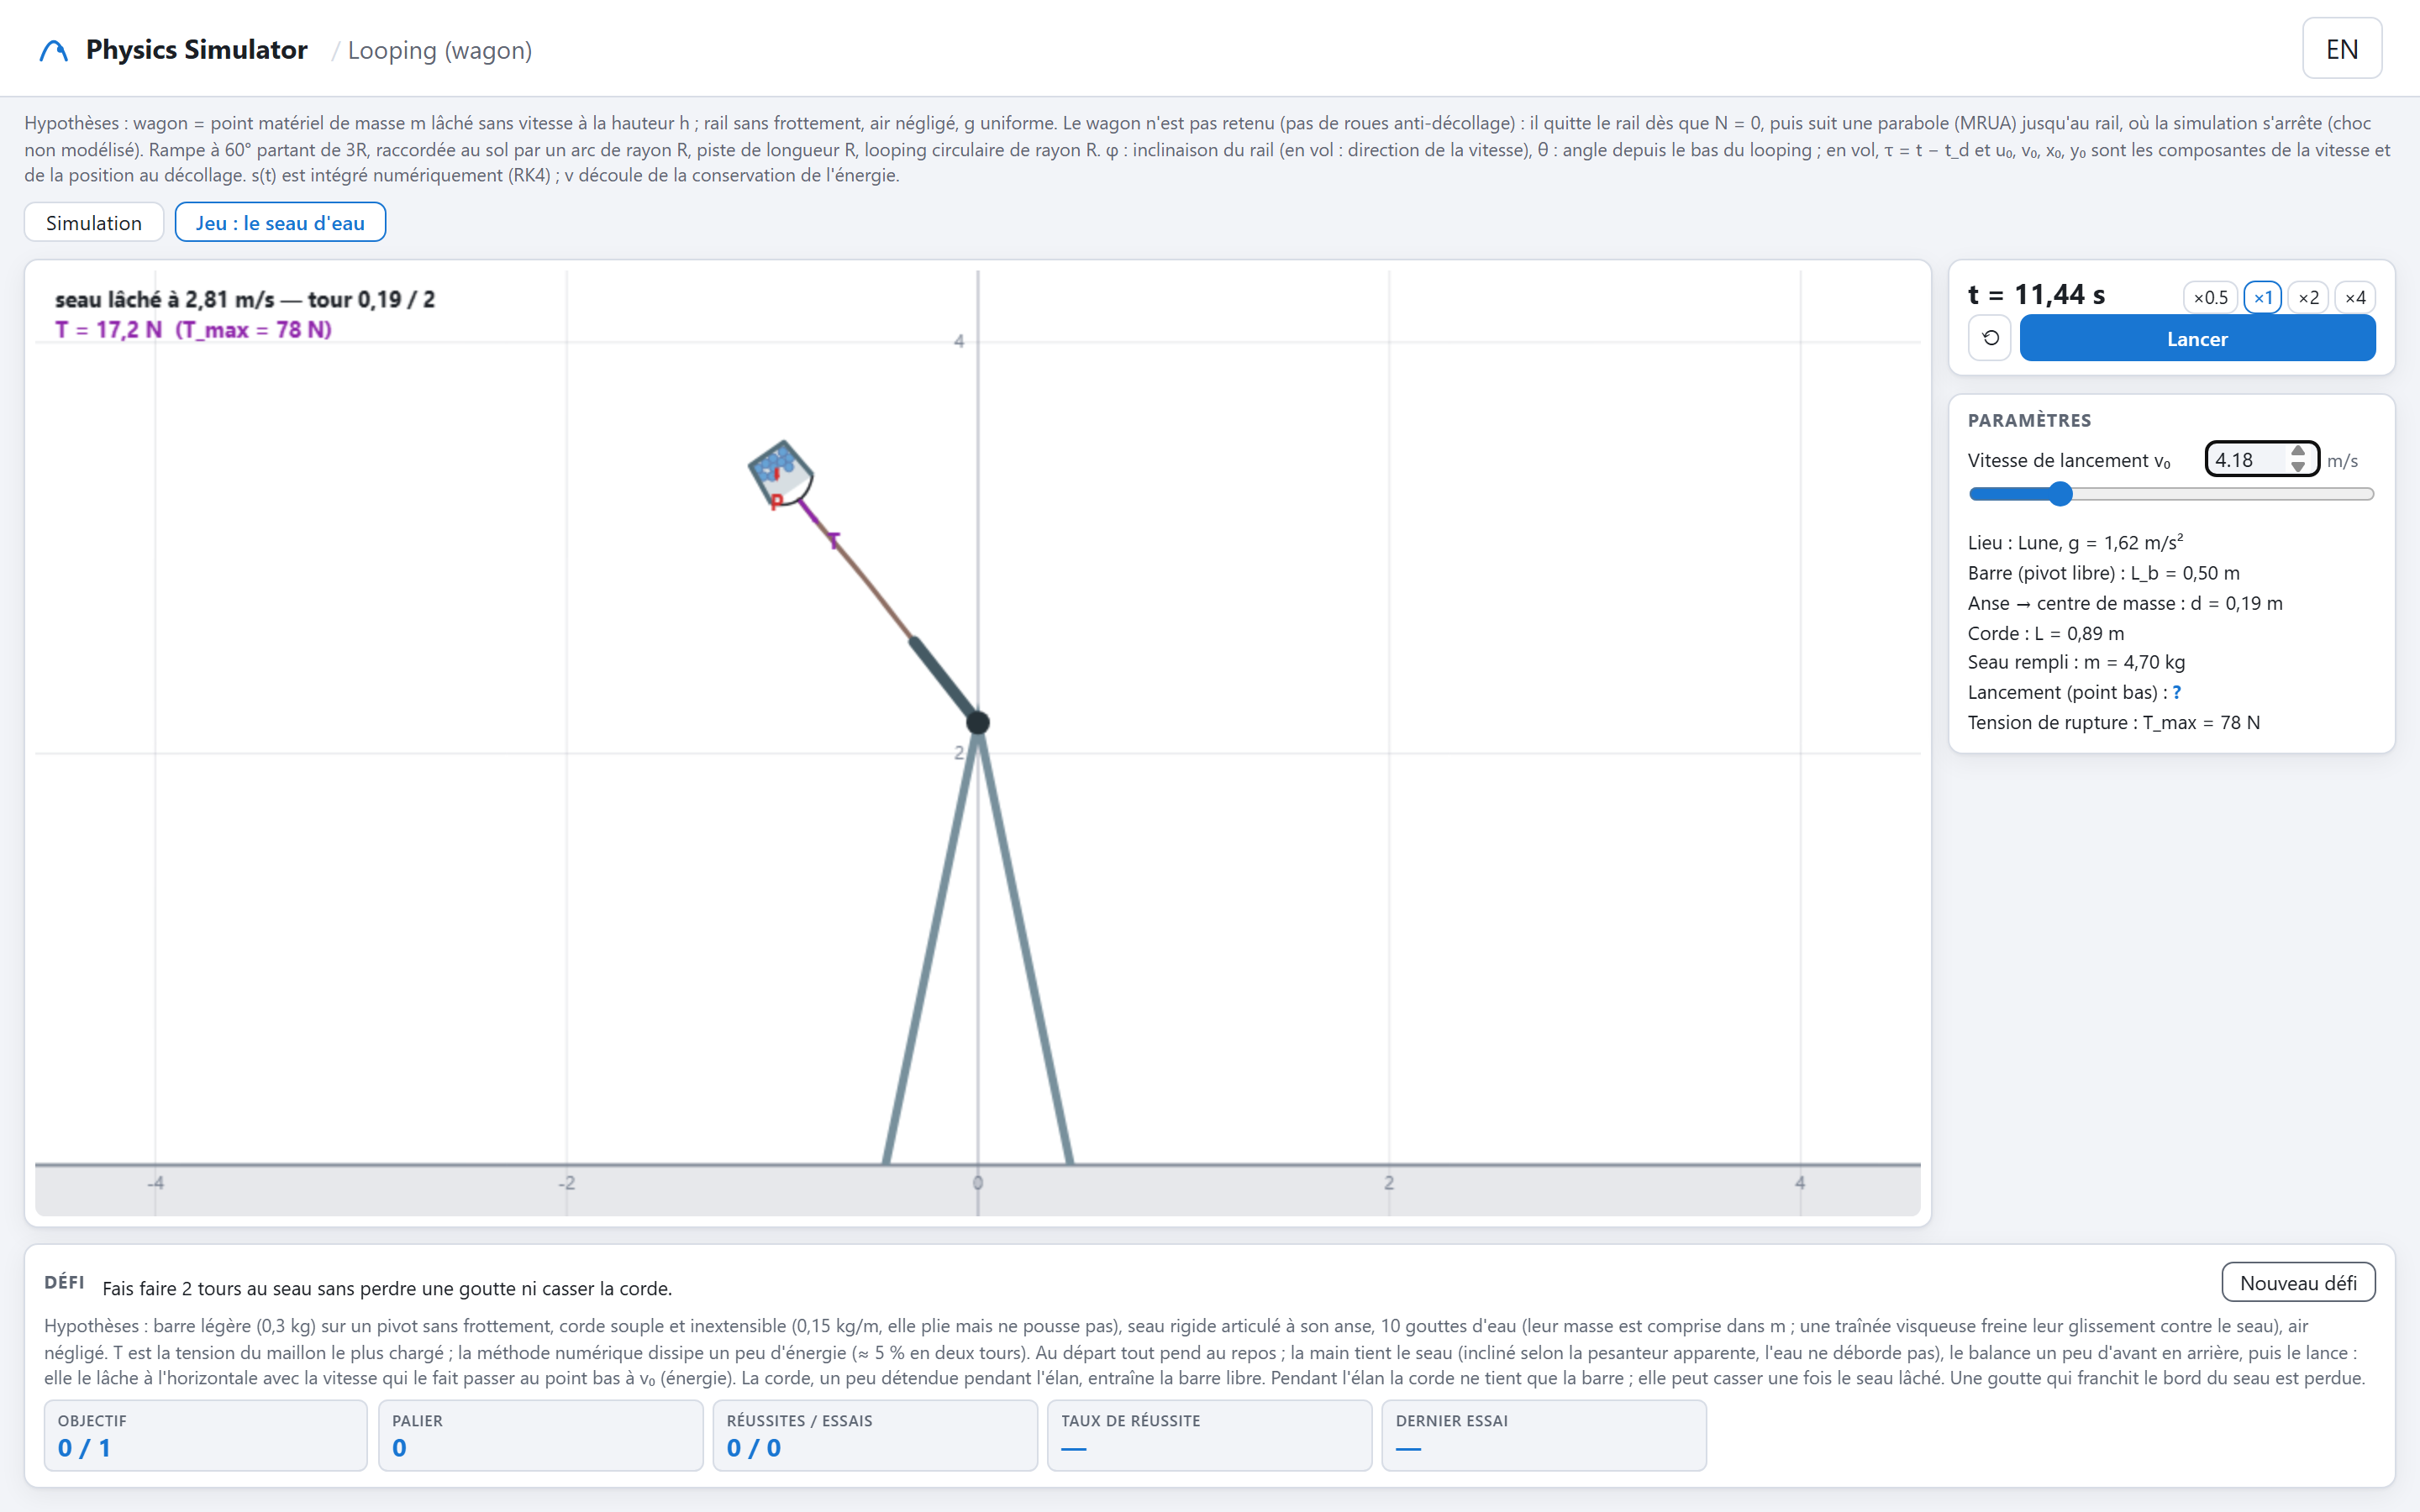
\includegraphics[width=\linewidth]{figures/captures/jeu-ecran-complet.png}
  \caption{Mode jeu du looping sur un écran de \(1440 \times 900\) pixels : scène
    fixe, réglage de la seule grandeur libre et données du défi à droite, panneau
    des statistiques et hypothèses en bas.}
\end{figure}

\begin{arediger}{2 à 4 pages}
Une capture par exercice (tir parabolique, pendule, MCU, looping
historique), avec une légende d'une ligne. Les captures se régénèrent avec
\fichier{outils/captures.cjs} (à étendre aux autres pages).
\end{arediger}


\end{document}
